\documentclass[dvipdfmx]{jsreport}
\usepackage{docmute}
\usepackage{graphicx, url, algorithm, algorithmic, float, booktabs, listings, color, pdfpages, amsmath, amssymb, latexsym, mathtools, ascmac, amsfonts, amsthm}
\lstset{
  basicstyle={\ttfamily},
  identifierstyle={\small},
  commentstyle={\smallitshape},
  keywordstyle={\small\bfseries},
  ndkeywordstyle={\small},
  stringstyle={\small\ttfamily},
  frame={tb},
  breaklines=true,
  columns=[l]{fullflexible},
  numbers=left,
  xrightmargin=0zw,
  xleftmargin=3zw,
  numberstyle={\scriptsize},
  stepnumber=1,
  numbersep=1zw,
  lineskip=-0.5ex
}
\usepackage[table,xcdraw]{xcolor}
\newtheorem{theo}{定理}[chapter]
\newtheorem{defi}{定義}[chapter]
\newtheorem{lemm}{補題}[chapter]
\newtheorem{prop}{命題}[chapter]
\newtheorem{coro}{系}[chapter]
\newcommand{\red}[1]{\textcolor{red}{#1}}
\newcommand{\blue}[1]{\textcolor{blue}{#1}}
\newcommand{\green}[1]{\textcolor{green}{#1}}
\renewcommand{\baselinestretch}{1.1}
\usepackage{mathrsfs}
\usepackage{bm}
\def\qed{\hfill $\Box$}
\usepackage{tikz}
\usetikzlibrary{intersections, calc, arrows}
\renewcommand\proofname{\bf 証明}

\title{最適化 復習}
\author{Kosuke Toda}
\date{}
\begin{document}
\maketitle

%%%%%%%%%%%% 目次 %%%%%%%%%%%%%%%%%%%%%%%%%%%%%%%%%%%%%%%%%%%%%%%%%%%%
\tableofcontents
\pagenumbering{arabic}


\chapter{まえがき}
様々な問題に対して,最も効率的になるように意思決定をする手法としてオペレーションズ・リサーチ(OR)というものがある~\cite{or}.これは,現実の問題を数理モデルに置換し,問題を解決する.最適化理論(optimization theory)は,ORの基礎理論の1つであり,理論だけでなく,現実の問題を解くための手法を提供してきた~\cite{opt}.本資料では,特に連続最適化に焦点を当てる.

%%%%%%%%%%%% 数学的準備 %%%%%%%%%%%%%%%%%%%%%%%%%%%%%%%%%%%%%%%%%%%%%%%%%%%
\documentclass{jsreport}
\usepackage{graphicx, url, algorithm, algorithmic, float, booktabs, listings, color, pdfpages, amsmath, amssymb, latexsym, mathtools, ascmac, amsfonts, amsthm}
\lstset{
  basicstyle={\ttfamily},
  identifierstyle={\small},
  commentstyle={\smallitshape},
  keywordstyle={\small\bfseries},
  ndkeywordstyle={\small},
  stringstyle={\small\ttfamily},
  frame={tb},
  breaklines=true,
  columns=[l]{fullflexible},
  numbers=left,
  xrightmargin=0zw,
  xleftmargin=3zw,
  numberstyle={\scriptsize},
  stepnumber=1,
  numbersep=1zw,
  lineskip=-0.5ex
}
\usepackage[table,xcdraw]{xcolor}
\newtheorem{theo}{定理}[chapter]
\newtheorem{defi}{定義}[chapter]
\newtheorem{lemm}{補題}[chapter]
\newtheorem{prop}{命題}[chapter]
\newtheorem{coro}{系}[chapter]
\newcommand{\red}[1]{\textcolor{red}{#1}}
\newcommand{\blue}[1]{\textcolor{blue}{#1}}
\newcommand{\green}[1]{\textcolor{green}{#1}}
\renewcommand{\baselinestretch}{1.1}
\usepackage{mathrsfs}
\usepackage{bm}
\def\qed{\hfill $\Box$}
\usepackage{tikz}
\usetikzlibrary{intersections, calc, arrows}
\renewcommand\proofname{\bf 証明}

\begin{document}
\chapter{数学的準備}
\section{諸定義}
$n$次元実数空間$\mathbb{R}^n$を考える.
\begin{itemize}
  \item $\varepsilon$-近傍
  \begin{itemize}
    \item $B(x, \varepsilon) = \{\bm{y} \in \mathbb{R}^n \, | \, \|\bm{y} - \bm{x} \| < \varepsilon\}$
    \item ただし,$\|\cdot\|$はユークリッドノルムであり,
    $\|\bm{x}\| = (\bm{x}^{\mathrm{T}}\bm{x})^{1/2}$である.
  \end{itemize}
  \item $X \subseteq \mathbb{R}^n$が開集合(open set)である
  \begin{itemize}
    \item $\forall \bm{x} \in X, \, \exists \varepsilon > 0; \, B(\bm{x}, \varepsilon) \subseteq X$
  \end{itemize}
  \item $X \subseteq \mathbb{R}^n$が閉集合(closed set)である
  \begin{itemize}
    \item $X$の補集合$X^\mathrm{c}$が開集合である.
  \end{itemize}
  \item $\bm{x}$が$X \subseteq \mathbb{R}^n$の内点(interior point)である
  \begin{itemize}
    \item $\bm{x} \in X \subseteq \mathbb{R}^n$に対して,
    $\exists \varepsilon > 0; \, B(\bm{x}, \varepsilon) \subseteq X$が成立する.
  \end{itemize}
  \item $X$の内部(interior),$\mathrm{Int}(X)$
  \begin{itemize}
    \item $X \subseteq \mathbb{R}^n$の内点の集合.
  \end{itemize}
  \item $\bm{x}$が$X \subseteq \mathbb{R}^n$の触点(contact point)である
  \begin{itemize}
    \item $\bm{x} \in X \subseteq \mathbb{R}^n$に対して,$\forall \varepsilon > 0; \, B(\bm{x}, \varepsilon) \cap X \neq \emptyset$が成立する.
  \end{itemize}
  \item $X$の閉包(closure),$\mathrm{Cl}(X)$
  \begin{itemize}
    \item $X \subseteq \mathbb{R}^n$の触点の集合.
    \item $X$を含む最小の閉集合.
  \end{itemize}
  \item $X$の境界(boundary),$\mathrm{Bd}(X)$
  \begin{itemize}
    \item $\mathrm{Bd}(X) = \mathrm{Cl}(X) \setminus \mathrm{Int}(X)$.
  \end{itemize}
  \item $\bm{x}$は$X$の集積点である
  \begin{itemize}
    \item 任意の$\varepsilon > 0$に対して,$B(\bm{x}, \varepsilon) \cap X$が$\bm{x}$と異なる要素を含む.
  \end{itemize}
  \item 孤立点(isolated point)
  \begin{itemize}
    \item $X$の集積点でない$X$の触点
  \end{itemize}
  \item $X$が有界である(bounded)
  \begin{itemize}
    \item $\exists \varepsilon > 0; \, X \subseteq B(\bm{0}, \varepsilon)$.
  \end{itemize}
  \item 収束
  \begin{itemize}
    \item 点列$\{\bm{x}^i\}, \, i = 1, 2, \ldots$を考える.
    $\forall \varepsilon > 0, \, \exists I_{\varepsilon}; \; \|\bm{x}^i - \bm{x}\| < \varepsilon, \, i \geq I_{\varepsilon}$となる点$\bm{x}$が存在するとき,$\bm{x}$は点列$\{\bm{x}^i\}$の極限(limit)といい,点列$\{\bm{x}^i\}$は$\bm{x}$に収束する(converge)という.
  \end{itemize}
  \item 点列$\{\bm{x}^i\}$の集積点
  \begin{itemize}
    \item $\{\bm{x}^i\}$の部分点列$\{\bm{x}^{l_i}\}$が点$\bm{x}$に収束するとき,点$\bm{x}$を点列$\{\bm{x}^i\}$の集積点という.
  \end{itemize}
\end{itemize}

有界閉集合$X \subseteq \mathbb{R}^n$について,$\{\bm{x}^i\} \subseteq X$なる無限点列は少なくとも1つの集積点をもつ.

\section{関数}
\begin{itemize}
  \item 連続性
  \begin{itemize}
    \item 関数$\bm{f}: X \rightarrow \mathbb{R}^m$を考える($X \subseteq R^n$).
    \begin{equation}
      \forall \epsilon > 0, \exists \delta > 0; \, \|\bm{x} - \bm{x}\| < \delta \Rightarrow \|\bm{f}(\bm{x}) - \bm{f}(\bm{x}^0) \| < \varepsilon \nonumber
    \end{equation}
    が成立するとき,$\bm{f}$は点$\bm{x}^0$で連続(continuous)であるという.
    \item 任意の$\bm{x} \in X$で連続となるとき,関数$\bm{f}$は$X$で連続という.
  \end{itemize}
  \item 実数値関数
  \begin{itemize}
    \item 値域が実数集合の関数$f: X \rightarrow \mathbb{R}$.
  \end{itemize}
  \item 実数値関数のクラス
  \begin{itemize}
    \item $f: X \rightarrow \mathbb{R}$($X \subseteq \mathbb{R}^n$は開集合)を考える.
    \item $f$が連続であるとき,$X$上で$C^0$級と呼ばれ,$f \in C^0$と記す.
    \item $f \in C^0$で,$\partial f(\bm{x}) / \partial x_i, \, i = 1, 2, \ldots, n$が存在し,連続であれば,$f$は$X$上で$C^1$級と呼ばれ,$f \in C^1$と表す.
    \item $f \in C^1$で,$\partial^2 f(\bm{x}) / \partial x_i \partial x_j, \, i,j = 1, 2, \ldots, n$が存在し,連続であれば,$f$は$X$上で$C^2$級と呼ばれ,$f \in C^2$と表す.
    \item 以後$C^k$級も同様に定義される.
  \end{itemize}
  \item 勾配ベクトル$\nabla f(\bm{x})$
    \begin{equation}
      \nabla f(\bm{x}) = \left(\frac{\partial f(\bm{x})}{\partial x_1}, \frac{\partial f(\bm{x})}{\partial x_2}, \cdots, \frac{\partial f(\bm{x})}{\partial x_n}\right) \nonumber
    \end{equation}
  \item ヘッセ行列$H(\bm{x}) = \nabla^2 f(\bm{x})$
  \begin{equation}
    \nabla^2 f(\bm{x}) = \left(
    \begin{array}{cccc}
      \displaystyle \frac{\partial^2 f(\bm{x})}{{\partial x_1}^2} & \displaystyle \frac{\partial^2 f(\bm{x})}{\partial x_1 \partial x_2} & \displaystyle \cdots & \displaystyle \frac{\partial^2 f(\bm{x})}{\partial x_1 \partial x_n} \\
      \displaystyle \frac{\partial^2 f(\bm{x})}{\partial x_2 \partial x_1} & \displaystyle \frac{\partial^2 f(\bm{x})}{{\partial x_2}^2} & \displaystyle \cdots & \displaystyle \frac{\partial^2 f(\bm{x})}{\partial x_2 \partial x_n} \\
      \vdots & \vdots & \ddots & \vdots \\
      \displaystyle \frac{\partial^2 f(\bm{x})}{\partial x_n \partial x_1} & \displaystyle \frac{\partial^2 f(\bm{x})}{\partial x_n \partial x_2} & \displaystyle \cdots & \displaystyle \frac{\partial^2 f(\bm{x})}{{\partial x_n}^2}
    \end{array}
    \right) \nonumber
  \end{equation}
\end{itemize}

\paragraph{Weierstrassの定理}
有界閉集合$X \subseteq \mathbb{R}^n$上の連続な実数値関数$f(\bm{x})$は$X$内の点で最大値,最小値をとる.

\paragraph{平均値の定理}
$f: X \rightarrow \mathbb{R} \, (X \subseteq \mathbb{R}^n), \, f \in C^1, \, \bm{x}^1, \bm{x}^2 \in X$に対して,
\begin{equation}
  f(\bm{x}^1) = f(\bm{x}^2) + \nabla f(\theta \bm{x}^1 + (1 - \theta) \bm{x}^2)^{\mathrm{T}}(\bm{x}^1 - \bm{x}^2) \nonumber
\end{equation}
を満たす$\theta \in (0, 1)$が存在する.

(注)関数$f: I \rightarrow \mathbb{R} \, (I \subseteq \mathbb{R}), \, f \in C^1, \, x_1, x_2 \in I$に対しては,
\begin{equation}
  f(x_1) = f(x_2) + f^{\prime}(\theta x_1 + (1-\theta)x_2)(x_1 - x_2) \nonumber
\end{equation}
を満たす$\theta \in (0, 1)$が存在する.これは,点$x_1, x_2 \in I$を結ぶ線分内に,$f(x_1), f(x_2)$を結ぶ直線と同じ傾きとなる接線を持つ点$c = \theta x_1 + (1-\theta)x_2, \, \theta \in (0, 1)$が存在することに相当する.

\paragraph{Taylorの定理}
$f: X \rightarrow \mathbb{R} \, (X \subseteq \mathbb{R}^n), \, f \in C^2, \, \bm{x}^1, \bm{x}^2 \in X$に対して,
\begin{equation}
  f(\bm{x}^1) = f(\bm{x}^2) + \nabla f(\bm{x}^2)^{\mathrm{T}} (\bm{x}^1 - \bm{x}^2)^{\mathrm{T}} + \frac{1}{2} (\bm{x}^1 - \bm{x}^2)^{\mathrm{T}} \nabla^2 f(\bm{x}^2) (\bm{x}^1 - \bm{x}^2) + o(\|\bm{x}^1 - \bm{x}^2 \|^2) \nonumber
\end{equation}
が成立する.ただし,$o$は$\lim\limits_{t \rightarrow 0} o(t) / t = 0$なる関数である.
同様に,$f \in C^1$に対して,
\begin{equation}
    f(\bm{x}^1) = f(\bm{x}^2) + \nabla f(\bm{x}^2)^{\mathrm{T}} (\bm{x}^1 - \bm{x}^2)^{\mathrm{T}} + o(\|\bm{x}^1 - \bm{x}^2 \|^1) \nonumber
\end{equation}
が成立する.

(注)関数$f: I \rightarrow \mathbb{R} \, (I \subseteq \mathbb{R}), \, f \in C^1, \, x_1, x_2 \in I$に対しては,
\begin{equation}
  f(x_1) = f(x_2) + f^{\prime}(x_2)(x_1 - x_2) + \frac{f^{\prime \prime}(x_2)}{2}(x_1 - x_2)^2 + o((x_1 - x_2)^2) \nonumber
\end{equation}
\begin{equation}
  f(x_1) = f(x_2) + f^{\prime}(x_2)(x_1 - x_2) + o(x_1 - x_2) \nonumber
\end{equation}
が成立する.$o$を用いずに表すと,
\begin{equation}
  f(x_1) = f(x_2) + f^{\prime}(x_2)(x_1 - x_2) + \frac{f^{\prime \prime}(x_2)}{2}(x_1 - x_2)^2 + \cdots + \frac{f^{(n - 1)}(x_2)}{(n - 1)!}(x_1 - x_2)^{n - 1} + R_n \nonumber
\end{equation}
\begin{equation}
  R_n \coloneqq \frac{f^{(n)}(\theta x_1 + (1 - \theta)x_2)}{n!}(x_1 - x_2)^n \nonumber
\end{equation}
を満たす$\theta \in (0, 1)$が存在する.$n = 1$のときは平均値の定理.つまり,Taylorの定理は平均値の定理の一般化と考えることができる.

\paragraph{陰関数の定理}
$h_i: \mathbb{R}^n \rightarrow \mathbb{R}, \, \bm{x}^0 = (x_1^0, x_1^0, \ldots, x_n^0)^{\mathrm{T}} \in \mathbb{R}^n$の近傍で,$h_i \in C^p \, (p \geq 1)$
\begin{equation}
  h_i(\bm{x}^0) = 0, \, i = 1, 2, \ldots, m \nonumber
\end{equation}
が成立するとする.このとき,ヤコビ行列(Jacobian matrix)
\begin{equation}
  J(\bm{x}^0) = \left(
  \begin{array}{ccc}
    \displaystyle \frac{\partial h_1(\bm{x}^0)}{\partial x_1} & \cdots & \displaystyle \frac{\partial h_1(\bm{x}^0)}{\partial x_m} \\
    \vdots & \vdots & \vdots \\
    \displaystyle \frac{\partial h_m(\bm{x}^0)}{\partial x_1} & \cdots & \displaystyle \frac{\partial h_m(\bm{x}^0)}{\partial x_m}
  \end{array}
  \right) \nonumber
\end{equation}
が正則ならば,ある$\varepsilon > 0$に対して$\hat{\bm{x}}^0 = (x_{m + 1}^0, \ldots, x_n^0)^{\mathrm{T}} \in \mathbb{R}^{n - m}$の近傍$U = B(\hat{\bm{x}}^0, \varepsilon)$が存在し,$\hat{\bm{x}} \in U$に対して,
\begin{enumerate}
  \item $\phi_i \in C^p, \, i = 1, 2, \ldots, m$
  \item $x_i = \phi(\hat{\bm{x}}), \, i = 1, 2, \ldots, m$
  \item $h_i(\phi_1(\hat{\bm{x}}), \phi_2(\hat{\bm{x}}), \ldots, \phi_m(\hat{\bm{x}}), \hat{\bm{x}}) = 0, i = 1, 2, \ldots, m$
\end{enumerate}
となる陰関数(implicit function)$\phi_i, \, i = 1, 2, \ldots, m$が存在する\footnote{解析学の教科書では,陰関数が唯一存在すると記されている.}.

(注) 2変数関数を考える.関数$f: \Omega \rightarrow \mathbb{R} \, (\Omega \subseteq \mathbb{R}^2), \, f \in C^p, \, p \geq 1, \, (x_1, x_2) \in \Omega$とする.$f(x_1, x_2) = 0$のとき,$x = x_1$を含む開区間$I$および$I$上で定義された$C^p$級の関数$\phi$がただ1つ存在し,$\phi(x_1) = x_2$および
\begin{equation}
  u(x) \coloneqq f(x, \phi(x)) = 0 \; \; (\forall x \in I) \nonumber
\end{equation}
が成立する.

\section{凸集合}
$X \subseteq \mathbb{R}^n$とする.$\forall \bm{x}^1, \bm{x}^2 \in X, \, \forall \lambda \in [0, 1]$に対して,$\lambda \bm{x}^1 + (1 - \lambda)\bm{x}^2 \in X$が成立するとき,$X$は凸集合(convex set)である
\footnote{2点$\bm{x}^1, \bm{x}^2$を結ぶ線分上の任意の内分点は,$x_{\lambda} = \lambda \bm{x}^1 + (1 - \lambda)\bm{x}^2, \, \lambda \in [0, 1]$と書ける.}.

\begin{lemm}\label{lemm:convex}
  $X_1, X_2, \ldots \subseteq \mathbb{R}^n$を凸集合とすると,$\bigcap \limits_{i = 1, 2, \ldots} X_i$も凸集合となる.
\end{lemm}

\begin{lemm}[分離超平面の存在]\label{lemm:hyperplane1}
  $X \subseteq \mathbb{R}^n$を空でない閉凸集合,$\bm{y} \notin X$とする.このとき,
  \begin{equation}
    \bm{a}^{\mathrm{T}}\bm{x} \geq b > \bm{a}^{\mathrm{T}}\bm{y}, \; \forall x \in X \nonumber
  \end{equation}
  となる分離超平面(separating hyperplane)$\{\bm{x} \in \mathbb{R}^n \, | \, \bm{a}^{\mathrm{T}} \bm{x} = b\} \; (\bm{a} \neq \bm{0})$が存在する.
\end{lemm}


\begin{lemm}\label{lemm:hyperplane2}
  $X \subseteq \mathbb{R}^n$を空でない凸集合,$\bm{y} \in \mathrm{Bd}(X)$とする.このとき,
  \begin{equation}
    \bm{a}^{\mathrm{T}} \bm{x} \geq \bm{a}^{\mathrm{T}} \bm{y}, \, \forall \bm{x} \in X \nonumber
  \end{equation}
  なる$\bm{a} \neq \bm{0}$が存在する.
\end{lemm}

\end{document}


%%%%%%%%%%%% 最適化問題の定式化 %%%%%%%%%%%%%%%%%%%%%%%%%%%%%%%%%%%%%%%%%%%%%%%%%%%
\documentclass{jsreport}
\usepackage{graphicx, url, algorithm, algorithmic, float, booktabs, listings, color, pdfpages, amsmath, amssymb, latexsym, mathtools, ascmac, amsfonts, amsthm}
\lstset{
  basicstyle={\ttfamily},
  identifierstyle={\small},
  commentstyle={\smallitshape},
  keywordstyle={\small\bfseries},
  ndkeywordstyle={\small},
  stringstyle={\small\ttfamily},
  frame={tb},
  breaklines=true,
  columns=[l]{fullflexible},
  numbers=left,
  xrightmargin=0zw,
  xleftmargin=3zw,
  numberstyle={\scriptsize},
  stepnumber=1,
  numbersep=1zw,
  lineskip=-0.5ex
}
\usepackage[table,xcdraw]{xcolor}
\newtheorem{theo}{定理}[chapter]
\newtheorem{defi}{定義}[chapter]
\newtheorem{lemm}{補題}[chapter]
\newtheorem{prop}{命題}[chapter]
\newtheorem{coro}{系}[chapter]
\newcommand{\red}[1]{\textcolor{red}{#1}}
\newcommand{\blue}[1]{\textcolor{blue}{#1}}
\newcommand{\green}[1]{\textcolor{green}{#1}}
\renewcommand{\baselinestretch}{1.1}
\usepackage{mathrsfs}
\usepackage{bm}
\def\qed{\hfill $\Box$}
\usepackage{tikz}
\usetikzlibrary{intersections, calc, arrows}
\renewcommand\proofname{\bf 証明}

\begin{document}

\chapter{最適化問題の定式化}
本章では,一般の最適化問題について定式化を行い,用語の定義を行う.
\section{最適化問題}
最適化問題を口語的に定義すると,「与えられた条件の下で何らかの関数を最小化,もしくは最大化する問題」である.最適化問題は以下のように定義される.ここでは,最小化問題を最適化問題とする.

基礎となる空間$X$,$S \subseteq \mathbb{R}^n$,$X$上で定義された関数$f: X \rightarrow \mathbb{R}$が与えられたとき,$f$を最小にする解$\bm{x} \in X \cap X$を求める問題を最適化問題(optimization problem),あるいは計画問題(programming problem)という.つまり,最適化問題は,(\ref{eq:opt})式で定義される問題である.
\begin{align}\label{eq:opt}
  \mathrm{minimize} &: f(\bm{x}) \nonumber\\
  \mathrm{subject \; to} &: \bm{x} \in S \cap X
\end{align}
例えば$X$として,$\mathbb{R}^n$や離散集合などが考えられる.
通常,$S$は関数$g_i: \mathbb{R}^n \rightarrow \mathbb{R}, \, i = 1, 2, \ldots, m$による不等式および等式制約を用いて,
\begin{equation}\label{eq:const}
  S = \{\bm{x} \in \mathbb{R}^n \, | \, g_i(\bm{x}) \leq 0, \, i = 1, 2, \ldots, l, \; g_i(\bm{x}) = 0, \, i = l + 1, \ldots, m\}
\end{equation}
と表現される.

\section{用語}
\begin{description}
  \item[$S \cap X$] 実行可能領域(feasible region)
  \begin{itemize}
    \item $S \cap X \neq \emptyset$ならば,実行可能(feasible)
    \item $S \cap X = \emptyset$ならば,実行不能(infeasible)
  \end{itemize}
  \item[$\bm{x} \in S \cap X$] 実行可能解(feasible solution)
\end{description}

実行可能解$\bm{x} \in S \cap X$のうち,目的関数値を最小にする解を最適解(optimal solution)という.つまり,最適化問題\ref{eq:opt}の最適解$\bm{x}^*$は,$\forall \bm{x} \in S \cap X, \, f(\bm{x}^*) \leq f(\bm{x})$を満たす$\bm{x}^* \in S \cap X$である.

最適化問題(\ref{eq:opt})において,最適解は常に存在するわけではない.実行不能であるとき,あるいはいくらでも目的関数値を小さくできる場合などでは,最適解は存在しない\footnote{実行不能であるとき,この問題を非有界(unbounded)であるといい,いくらでも目的関数値を小さくできる場合,この問題は発散する(divergent)という.}.

最適化問題は,基礎となる空間$X$,目的関数$f$,制約式(\ref{eq:const})における$g_i$により次のように分類される.
\begin{itemize}
  \item 非線形計画問題(nonlinear programming problem)
  \begin{itemize}
    \item $X = \mathbb{R}^n$
    \item $f$や$S$を定義する$g_i$に制限を置かない.
  \end{itemize}
  \item 線形計画問題(linear programming problem)
  \begin{itemize}
    \item $f, g_i$がすべて線形(1次関数).
  \end{itemize}
  \item 整数計画問題(integer programming problem)
  \begin{itemize}
    \item $X = \mathbb{Z}^n$
    \item $f, g_i$が線形.
    \item すべての変数が整数変数の全整数計画問題(all-integer programming problem),整数変数と実数変数が混在する混合整数計画問題(mixed-integer programming problem)に分類される.
  \end{itemize}
  \item 組合せ最適化問題(combinatorial optimization problem)
  \begin{itemize}
    \item 離散集合$X$に対する最適化問題.
    \item グラフ理論など.
  \end{itemize}
\end{itemize}

最適化問題(\ref{eq:opt})は,
\begin{equation}
  f^* = \inf_{\bm{x} \in S \cap X} f(\bm{x}) \nonumber
\end{equation}
を求める問題と解釈できる.$f^*$を最適値(optimal value)という.最適値$f^*$は常に定義され,最小化問題については,実行不能ならば$f^* = \infty$,発散するならば$f^* = -\infty$であり,最適解$\bm{x}^*$が存在するならば$f^* = f(\bm{x}^*)$である.

\end{document}


%%%%%%%%%%%% 非線形計画問題 %%%%%%%%%%%%%%%%%%%%%%%%%%%%%%%%%%%%%%%%%%%%%%%%%%%
\documentclass{jsreport}
\usepackage{graphicx, url, algorithm, algorithmic, float, booktabs, listings, color, pdfpages, amsmath, amssymb, latexsym, mathtools, ascmac, amsfonts, amsthm}
\lstset{
  basicstyle={\ttfamily},
  identifierstyle={\small},
  commentstyle={\smallitshape},
  keywordstyle={\small\bfseries},
  ndkeywordstyle={\small},
  stringstyle={\small\ttfamily},
  frame={tb},
  breaklines=true,
  columns=[l]{fullflexible},
  numbers=left,
  xrightmargin=0zw,
  xleftmargin=3zw,
  numberstyle={\scriptsize},
  stepnumber=1,
  numbersep=1zw,
  lineskip=-0.5ex
}
\usepackage[table,xcdraw]{xcolor}
\newtheorem{theo}{定理}[chapter]
\newtheorem{defi}{定義}[chapter]
\newtheorem{lemm}{補題}[chapter]
\newtheorem{prop}{命題}[chapter]
\newtheorem{coro}{系}[chapter]
\newcommand{\red}[1]{\textcolor{red}{#1}}
\newcommand{\blue}[1]{\textcolor{blue}{#1}}
\newcommand{\green}[1]{\textcolor{green}{#1}}
\renewcommand{\baselinestretch}{1.1}
\usepackage{mathrsfs}
\usepackage{bm}
\def\qed{\hfill $\Box$}
\usepackage{tikz}
\usetikzlibrary{intersections, calc, arrows}
\renewcommand\proofname{\bf 証明}

\begin{document}

\chapter{非線形計画問題とアルゴリズム}
この章では,非線形計画問題の最適性条件および最適化問題を解くアルゴリズムを述べる.
\section{非線形計画問題の最適性条件}
非線形計画問題においては,最適性の定義を次のように緩めることが多い.
\begin{itemize}
  \item $\bm{x}^*$は局所最小解(locally minimal solution)である.
  \begin{itemize}
    \item $\bm{x}^* \in S$に対し,ある近傍$B$が存在し,任意の$\bm{x} \in S \cap B$に対して$f(\bm{x}^*) \leq f(\bm{x})$が成立する.
  \end{itemize}
  \item $\bm{x}^*$は局所最大解(locally maximum solution)である.
  \begin{itemize}
    \item $\bm{x}^* \in S$に対し,ある近傍$B$が存在し,任意の$\bm{x} \in S \cap B$に対して$f(\bm{x}^*) \geq f(\bm{x})$が成立する.
  \end{itemize}
\end{itemize}

ここでは,最小化問題を基本としているので,局所最小解を局所最適解(locally optimal solution)ともいう.また,本来の最適解を大域最適解(globally optimal solution)という.
まず,局所最適解の必要条件,十分条件について述べ,局所最適解が大域最適解になる場合について述べる.

\subsection{制約なし問題の最適性条件}
最適化問題として,(\ref{eq:opt_nonl_nonc})を考える.
\begin{align}\label{eq:opt_nonl_nonc}
  \mathrm{minimize} &: f(\bm{x}) \nonumber\\
  \mathrm{subject \; to} &: \bm{x} \in \mathbb{R}^n
\end{align}
ただし,$f$は任意の非線形関数であり,適当な微分可能性を仮定する.

問題(\ref{eq:opt_nonl_nonc})の最適性の必要条件として,次の2つの定理を示す.
\begin{theo}\label{theo:opt_nonl_nonc_h_1}
  $f \in C^{1}$のとき,$\bar{\bm{x}} \in \mathbb{R}$が問題(\ref{eq:opt_nonl_nonc})の局所最適解であるための必要条件は,
  \begin{equation}
    \nabla f(\bar{\bm{x}}) = \bm{0} \nonumber
  \end{equation}
  となることである.
\end{theo}

\begin{theo}\label{theo:opt_nonl_nonc_h_2}
  $f \in C^2$のとき,$\bar{\bm{x}}$が問題(\ref{eq:opt_nonl_nonc})の局所最適解であるための必要条件は,
  \begin{equation}
    \nabla f(\bar{\bm{x}}) = \bm{0} \nonumber
  \end{equation}
  かつ,$\bar{\bm{x}}$におけるヘッセ行列$H(\bar{\bm{x}})$が半正定値,すなわち,
  \begin{equation}
    \bm{d}^{\mathrm{T}} H(\bar{\bm{x}}) \bm{d} \geq 0, \; \forall \bm{d} \in \mathbb{R}^n \nonumber
  \end{equation}
  が成立することである.
\end{theo}

さらに,局所最適解の十分条件は,定理\ref{theo:opt_nonl_nonc_j}で与えられる.
\begin{theo}\label{theo:opt_nonl_nonc_j}
  $f \in C^2$のとき,$\bar{\bm{x}}$が問題(\ref{eq:opt_nonl_nonc})の局所最適解であるための十分条件は,
  \begin{equation}
    \nabla f(\bar{\bm{x}}) = \bm{0} \nonumber
  \end{equation}
  かつヘッセ行列$H(\bar{\bm{x}})$が正定値,すなわち,
  \begin{equation}
    \bm{d}^{\mathrm{T}} H(\bar{\bm{x}}) \bm{d} > 0, \; \forall \bm{d} \in \mathbb{R}^n, \; \bm{d} \neq \bm{0} \nonumber
  \end{equation}
  が成立することである.
\end{theo}




\end{document}


%%%%%%%%%%%% 線形計画問題 %%%%%%%%%%%%%%%%%%%%%%%%%%%%%%%%%%%%%%%%%%%%%%%%%%%
\documentclass{jsreport}
\usepackage{graphicx, url, algorithm, algorithmic, float, booktabs, listings, color, pdfpages, amsmath, amssymb, latexsym, mathtools, ascmac, amsfonts, amsthm}
\lstset{
  basicstyle={\ttfamily},
  identifierstyle={\small},
  commentstyle={\smallitshape},
  keywordstyle={\small\bfseries},
  ndkeywordstyle={\small},
  stringstyle={\small\ttfamily},
  frame={tb},
  breaklines=true,
  columns=[l]{fullflexible},
  numbers=left,
  xrightmargin=0zw,
  xleftmargin=3zw,
  numberstyle={\scriptsize},
  stepnumber=1,
  numbersep=1zw,
  lineskip=-0.5ex
}
\usepackage[table,xcdraw]{xcolor}
\newtheorem{theo}{定理}[chapter]
\newtheorem{defi}{定義}[chapter]
\newtheorem{lemm}{補題}[chapter]
\newtheorem{prop}{命題}[chapter]
\newtheorem{coro}{系}[chapter]
\newcommand{\red}[1]{\textcolor{red}{#1}}
\newcommand{\blue}[1]{\textcolor{blue}{#1}}
\newcommand{\green}[1]{\textcolor{green}{#1}}
\renewcommand{\baselinestretch}{1.1}
\usepackage{mathrsfs}
\usepackage{bm}
\def\qed{\hfill $\Box$}
\usepackage{tikz}
\usetikzlibrary{intersections, calc, arrows}
\renewcommand\proofname{\bf 証明}

\begin{document}

\chapter{線形計画問題}
本章では,線形計画問題の定式化,最適性,およびアルゴリズムについて述べる.
\section{線形計画問題の例}
線形計画問題の例として,しばしば生産計画問題が挙げられる.例えば,次のような問題である.
\begin{description}
  \item[生産計画問題]
  A社では,2種類の製品$P_1, \, P_2$を同じ原料から生産している.$P_1$ 1トン生産するのに要する原料は2.5トン,電力は5kwh,労力は3人時,$P_2$ 1トン生産するのに要する原料は5トン,電力は6kwh,労力は2人時である.1日の原料,電力,労力の使用可能量は,それぞれ350トン,450kwh,240人時である.$P_1, \, P_2$ 1トン当たりの粗利益は,それぞれ,4万円,5万円である.このとき,総粗利益を最大にするには,$P_1, \, P_2$を何トンずつ生産すればよいか.
\end{description}

$P_1, \, P_2$の1日の生産量(トン)をそれぞれ$x_1, \, x_2$とする.この問題は表\ref{tab:product_plan}のように表される.
\begin{table}[htb]
  \centering
    \caption{生産計画問題}
    \begin{tabular}{c|c|c|c}
       & $P_1$ & $P_2$ &  \\ \hline
      原料 & $2.5x_1$ & $5x_2$ & $350$ \\ \hline
      電力 & $5x_1$ & $6x_2$ & $450$ \\ \hline
      労力 & $3x_1$ & $2x_2$ & $240$ \\ \hline
      粗利益 & $4x_1$ & $5x_2$ & \\
    \end{tabular}
    \label{tab:product_plan}
\end{table}

以上より,この生産計画問題は次の線形計画問題となる.
\begin{align}\label{eq:product_plan}
  \mathrm{maximize} \; \; &4x_1 + 5x_2 \nonumber \\
  \mathrm{subject \; to} \; \; &2.5x_1 + 5x_2 \leq 350 \nonumber \\
  &5x_1 + 6x_2 \leq 450 \\
  &3x_1 + 2x_2 \leq 240 \nonumber \\
  &x_1, x_2 \geq 0 \nonumber
\end{align}

\section{線形計画問題の最適解}
\ref{sec:convex_prob}節で述べたように,線形計画問題の実行可能領域は凸多面体であり,目的関数も線形(凸関数)であるので,線形計画問題は凸計画問題である.線形計画問題の最適解は,実行可能領域の多面体の頂点に存在する.この事実を確認する.
一般に多面体$X$は,すべての頂点からなる集合$V = \{\bm{v}_1, \bm{v}_2, \ldots, \bm{v}_p\}$を用いて,次のように表すことができる.
\begin{equation}
  X = \left\{\bm{x} \in \mathbb{R}^n \, | \, \bm{x} = \sum_{i = 1}^p k_i \bm{v}_i , \, \sum_{i = 1}^p k_i = 1, \, k_i \geq 0, \, i = 1, 2, \ldots, p \right\} \nonumber
\end{equation}

また,線形計画問題の目的関数は,$\bm{c}^{\mathrm{T}}\bm{x}$と表される.実行可能解$\bm{x} \in X$を考えると,$\sum_{i = 1}^p k_i = 1, \, k_i \geq 0, \, i = 1, 2, \ldots, p$を満たす$(k_1, k_2, \ldots, k_p)^{\mathrm{T}}$が存在して,
\begin{equation}
  \bm{x} = \sum_{i = 1}^p k_i \bm{v}_i \nonumber
\end{equation}
と表される.両辺に左から$\bm{c}^{\mathrm{T}}$を掛けると,
\begin{equation}
  \bm{c}^{\mathrm{T}} \bm{x} = \bm{c}^{\mathrm{T}} \left(\sum_{i = 1}^p k_i \bm{v}_i \right) = \sum_{i = 1}^p k_i \bm{c}^{\mathrm{T}} \bm{v}_i \nonumber
\end{equation}
となる.$\sum_{i = 1}^p k_i = 1, \, k_i \geq 0, \, i = 1, 2, \ldots, p$より,
\begin{equation}
  \min_{i = 1, 2, \ldots, p} \bm{c}^{\mathrm{T}} \bm{v}_i \leq \bm{c}^{\mathrm{T}} \bm{x} \leq \max_{i = 1, 2, \ldots, p} \bm{c}^{\mathrm{T}} \bm{v}_i \nonumber
\end{equation}
となる.$i = 1, 2, \ldots, p$について,$\bm{v}_i \in X$より,実行可能領域$X$での$\bm{c}^{\mathrm{T}}\bm{x}$の最大値および最小値を与える解の1つは,頂点集合$V$内にある.

\section{標準形の線形計画問題}
\subsection{線形計画問題の標準形}
変数が非負で等式制約条件しかもたない最小化問題を標準形(standard form)の線形計画問題という.すなわち,線形計画問題の標準形は,
\begin{align}\label{eq:standard}
  \mathrm{minimize} \; \; &\bm{c}^{\mathrm{T}}\bm{x} \nonumber \\
  \mathrm{subject \; to} \; \; &A\bm{x} = \bm{b} \\
  &\bm{x} \geq \bm{0} \nonumber
\end{align}
である.ただし,$\bm{c} = (c_1, c_2, \ldots, c_n)^{\mathrm{T}}, \, \bm{b} = (b_1, b_2, \ldots, b_m)^{\mathrm{T}}$はそれぞれ$n$次元,$m$次元の実数定ベクトルである.$A$は$m \times n \, (m \leq n)$の実数定行列である.$\bm{x} = (x_1, x_2, \ldots, x_n)^{\mathrm{T}}$は$n$次元の実数変数ベクトルであり,決定変数ベクトルと呼ばれる.

\subsection{標準形への変形}
\begin{description}
  \item[最大化問題の場合]
  線形計画問題が最大化問題の場合,つまり,
  \begin{equation}
    \mathrm{maximize} \; \; \bm{c}^{\mathrm{T}}\bm{x} \nonumber
  \end{equation}
  の場合,$\bm{d} = -\bm{c}$とすると,
  \begin{equation}
    \mathrm{maximize} \; \; \bm{c}^{\mathrm{T}}\bm{x} \Leftrightarrow \mathrm{minimize} \; \; \bm{d}^{\mathrm{T}}\bm{x} \nonumber
  \end{equation}
  と最小化問題に変形できる.
  \item[不等式条件$\leq$の場合]
  制約条件の1つが,
  \begin{equation}
    \bm{a}_i^{\mathrm{T}}\bm{x} \leq b_i \nonumber
  \end{equation}
  である場合,スラック変数(slack variable) $s \, (s \geq 0)$を導入して,
  \begin{equation}
    \bm{a}_i^{\mathrm{T}}\bm{x} \leq b_i \Leftrightarrow \bm{a}_i^{\mathrm{T}}\bm{x} + s = b_i, \; s \geq 0 \nonumber
  \end{equation}
  と等式条件に変形される.
  \item[不等号条件$\geq$の場合]
  制約条件の1つが,
  \begin{equation}
    \bm{a}_j^{\mathrm{T}}\bm{x} \geq b_j \nonumber
  \end{equation}
  である場合,サープラス変数(surplus variable) $t \, (t \geq 0)$を導入して,
  \begin{equation}
    \bm{a}_j^{\mathrm{T}}\bm{x} \leq b_j \Leftrightarrow \bm{a}_j^{\mathrm{T}}\bm{x} - t = b_j, \; t \geq 0 \nonumber
  \end{equation}
  と等式条件に変形される.
  \item[自由変数(非負条件の無い変数)が存在する場合]
  $x_k$に対して,$x_k \geq 0$という条件が存在せず,負の値も取る場合は,$x_k$を次の条件を満たす2つの変数$x_k^{+}$と$x_k^{-}$に分解して取り扱われる.
  \begin{equation}
    x_k = x_k^{+} - x_k^{-}, \; x_k^{+} \geq 0, x_k^{-} \geq 0 \nonumber
  \end{equation}
\end{description}

例えば,最適化問題(\ref{eq:product_plan})を標準形の線形計画問題に変形すると,(\ref{eq:product_plan_stand})になる.
\begin{align}\label{eq:product_plan_stand}
  \mathrm{minimize} \; \; &-4x_1 - 5x_2 \nonumber \\
  \mathrm{subject \; to} \; \; &2.5x_1 + 5x_2 + x_3 = 350 \nonumber \\
  &5x_1 + 6x_2 + x_4 = 450 \\
  &3x_1 + 2x_2 + x_5 = 240 \nonumber \\
  &x_1, x_2, x_3, x_4, x_5 \geq 0 \nonumber
\end{align}

\section{基底解と最適解}
\subsection{用語}
\begin{description}
  \item[基底行列]
  基底行列(basic matrix) $B$とは,制約条件の係数行列$A$の$m$個(制約条件数)の列ベクトルから作られる$m \times m$の正則行列のことをいう($|B| \neq 0$).
  \item[基底解]
  線形計画問題の基底解(basic solution)とは,ある基底行列$B$で選ばれなかった$(n - m)$個の列に対応する変数(非基底変数(nonbasic variable))を0とおき,選ばれた$m$個の変数(基底変数(basic variable))に対する正則な連立方程式
  \begin{equation}\label{eq:basic}
    B \left(
    \begin{array}{c}
      x_1^{B} \\
      x_2^{B} \\
      \vdots \\
      x_m^{B}
    \end{array}
    \right) = \bm{b}
  \end{equation}
  を解くことにより得られる一意的なベクトル$B^{-1}\bm{b}$のことをいう.
  \item[実行可能基底解]
  実行可能解であり,基底解である解を実行可能基底解(basic feasible solution)という.基底行列を$B$とすると,$B^{-1}\bm{b} \geq \bm{0}$のときに基底行列$B$に対応する基底解は実行可能基底解となる.
  \item[退化]
  基底解では,$m$個の基底変数のみが正の値を取りうるが,この$m$個の基底変数の内少なくとも1つが0となる基底解は,退化しているという.
\end{description}

\subsection{線形計画問題の基本定理}
標準形の線形計画問題(\ref{eq:standard})において,次の定理が成立する.
\begin{theo}[線形計画問題の基本定理]\label{theo:linear_th}
  標準形の線形計画問題(\ref{eq:standard})が与えられたとき,次の1, 2が成立する.
  \begin{enumerate}
    \item 実行可能解が存在するならば,必ず実行可能基底解が存在する.
    \item 最適解が存在するならば,実行可能基底解の中に最適解が存在する.
  \end{enumerate}
\end{theo}
定理\ref{theo:linear_th}より,線形計画問題の最適解を求めるには,基底解の中で,実行可能かつ最適なものを見つければよい\footnote{実行可能領域の端点を辿っていけば最適解に到達する.後述のシンプレックス法はこの考えに基づいている.}.

\subsection{基底形式}
標準形の線形計画問題
\begin{align}\label{eq:standard_re}
  \mathrm{minimize} \; \; &z = \bm{c}^{\mathrm{T}}\bm{x} \nonumber \\
  \mathrm{subject \; to} \; \; &A\bm{x} = \bm{b} \\
  &\bm{x} \geq \bm{0} \nonumber
\end{align}
において,$m \times n$行列$A$から$m$個の列を選び基底行列$B$とする.ただし,$B$は正則行列とする.残りの列からなる行列を$N$とする.列の順番と変数の順番を適当に変えることにより,
$A = (B, N), \bm{x} = (\bm{x}_B^{\mathrm{T}}, \bm{x}_{N}^{\mathrm{T}})^{\mathrm{T}}, \bm{c} = (\bm{c}_B^{\mathrm{T}}, \bm{c}_N^{\mathrm{T}})^{\mathrm{T}}$
と表すと,式(\ref{eq:standard_re})は,
\begin{align}\label{eq:standard_re_basic}
  \mathrm{minimize} \; \; &z = \bm{c}_B^{\mathrm{T}}\bm{x}_B + \bm{c}_N^{\mathrm{T}}\bm{x}_N \nonumber \\
  \mathrm{subject \; to} \; \; &B\bm{x}_B + N\bm{x}_N = \bm{b} \\
  &\bm{x}_B, \bm{x}_N \geq \bm{0} \nonumber
\end{align}
と表される.$\bm{x}_B$は基底変数ベクトル,$\bm{x}_N$は非基底変数ベクトル,
$\bm{x}_B$の各成分$x_j^B$は基底変数,
$\bm{x}_N$の各成分$x_j^N$は非基底変数と呼ばれる.$B$は正則より,目的関数から$\bm{x}_B$を消去すると,(\ref{eq:standard_re_basic})の問題は,
\begin{align}\label{eq:standard_re_equal}
  \mathrm{minimize} \; \; &z = \bm{c}_B^{\mathrm{T}}B^{-1}\bm{b} + (\bm{c}_N^{\mathrm{T}} - \bm{c}_B^{\mathrm{T}}B^{-1}N)\bm{x}_N \nonumber \\
  \mathrm{subject \; to} \; \; &\bm{x}_B + B^{-1}N\bm{x}_N = B^{-1}\bm{b} \\
  &\bm{x}_B, \bm{x}_N \geq \bm{0} \nonumber
\end{align}
と等価になる.(\ref{eq:standard_re_equal})の一部
\begin{align}\label{eq:basic_form}
  &z = \bm{c}_B^{\mathrm{T}}B^{-1}\bm{b} + (\bm{c}_N^{\mathrm{T}} - \bm{c}_B^{\mathrm{T}}B^{-1}N)\bm{x}_N \nonumber \\
  &\bm{x}_B + B^{-1}N\bm{x}_N = B^{-1}\bm{b}
\end{align}
は,基底形式(basic form)あるいは正準形(cannoncial form)と呼ばれる.このとき,基底行列は$B$であり,対応する基底解は
\begin{equation}\label{eq:basic_sol}
  \bm{x} = \left(
  \begin{array}{c}
    \bm{x}_B \\
    \bm{x}_N
  \end{array}
  \right) = \left(
  \begin{array}{c}
    B^{-1}\bm{b} \\
    \bm{0}
  \end{array}
  \right)
\end{equation}
となる.
以後,$\bar{\bm{c}}^{\mathrm{T}} = \bm{c}_N^{\mathrm{T}} - \bm{c}_B^{\mathrm{T}}B^{-1}N, \, \bar{N} = B^{-1}N, \, \bar{\bm{b}} = B^{-1}\bm{b}$と定める.
また,$\bar{\bm{c}}, \, \bar{N}, \, \bar{\bm{b}}$の各成分をそれぞれ,
$\bar{c}_{j}, \, \bar{a}_{ij}, \, \bar{b}_i$と表す.

(\ref{eq:basic_form})式を$\bar{\bm{c}}, \bar{N}, \bar{\bm{b}}$を用いて表すと,
\begin{align}\label{eq:basic_form_re}
  &z = \bm{c}_B^{\mathrm{T}}\bar{\bm{b}} + \bar{\bm{c}}^{\mathrm{T}}\bm{x}_N \nonumber \\
  &\bm{x}_B + \bar{N}\bm{x}_N = \bar{\bm{b}}
\end{align}
となる.(\ref{eq:standard_re_equal})式において,
\begin{equation}\label{eq:feasible_b}
  \bar{\bm{b}} = B^{-1}\bm{b} \geq \bm{0} \; \; (実行可能性)
\end{equation}
が成立すれば,(\ref{eq:basic_sol})式の基底解は実行可能解となる.(\ref{eq:feasible_b})が満たされると仮定する.

基底形式(\ref{eq:basic_form})のある非基底変数$x_r^N$の係数$\bar{c}_r$が負であれば,この非基底変数に正の値を取らせることにより,目的関数が改善できる\footnote{$\bar{c}_r < 0$ならば,$x_r^N > 0$を取ることで,実行可能性を維持したまま(\ref{eq:basic_form})式の$z$の値を小さくすることができる.}.逆に,すべての非基底変数$x_j^N$の係数$\bar{c}_j$が正,すなわち,
\begin{equation}\label{eq:opt_con}
  \bar{\bm{c}}^{\mathrm{T}} = \bm{c}_N^{\mathrm{T}} - \bm{c}_B^{\mathrm{T}}B^{-1}N \geq \bm{0}^{\mathrm{T}} \; \; (最適性)
\end{equation}
が成立すれば,この実行可能基底解は最適解の1つである.

次に,$\bar{c}_r$が負であるとき,実行可能性を維持する,つまり,$x_r^N$に正の値を取らせることが可能であるかどうかを考える.ここで,$x_r^N$以外の非基底変数$x_j^N$の値を0に固定する.このとき,
\begin{equation}\label{eq:x_B}
  \bm{x}_B = \bar{\bm{b}} -
  \left(
  \begin{array}{c}
    \bar{a}_{1r} \\
    \bar{a}_{2r} \\
    \vdots \\
    \bar{a}_{mr}
  \end{array}
  \right)x_r^N
\end{equation}
を満たせば,制約条件の最初の等式条件$\bm{x}_B + \bar{N}\bm{x}_N = \bar{\bm{b}}$を満足する.
実際,$\bm{x}_N = \left(0, \cdots, x_r^N, \cdots, 0 \right)^{\mathrm{T}}$
のとき,
\begin{equation}
  \bar{N} \bm{x}_N = \left(
  \begin{array}{ccccc}
    \bar{a}_{11} & \cdots & \bar{a}_{1r} & \cdots & \bar{a}_{1 n-m} \\
    \vdots & \ddots & \vdots & \ddots & \vdots \\
    \bar{a}_{m1} & \cdots & \bar{a}_{mr} & \cdots & \bar{a}_{m n-m}
  \end{array}
  \right) \left(
  \begin{array}{c}
    0 \\
    \vdots \\
    x_r^N \\
    \vdots \\
    0
  \end{array}
  \right) = \left(
  \begin{array}{c}
    \bar{a}_{1r} \\
    \bar{a}_{2r} \\
    \vdots \\
    \bar{a}_{mr}
  \end{array}
  \right)x_r^N \nonumber
\end{equation}
を満たす.さらに,非負条件を満たすには,$\bm{x}_B \geq \bm{0}$より,
\begin{equation}\label{eq:notminus}
  \bar{\bm{b}} -
  \left(
  \begin{array}{c}
    \bar{a}_{1r} \\
    \bar{a}_{2r} \\
    \vdots \\
    \bar{a}_{mr}
  \end{array}
  \right)x_r^N \geq \bm{0}
\end{equation}
が成立すればよい.もし,
\begin{equation}\label{eq:a_minus}
  \left(
  \begin{array}{c}
    \bar{a}_{1r} \\
    \bar{a}_{2r} \\
    \vdots \\
    \bar{a}_{mr}
  \end{array}
  \right) \leq \bm{0}
\end{equation}
が成立すれば,(\ref{eq:notminus})式より,実行可能性を損なうことなく$x_r^N$をいくらでも正に大きくすることができる.このとき,目的関数値をいくらでも小さくすることができるので,この解は非有解(unbounded solution)である.すなわち,最適解は存在しない.

一方,(\ref{eq:a_minus})式が成立しない場合,$\bar{a}_{ir}$のいくつかは正となる.(\ref{eq:notminus})式を満たすには,$\bar{a}_{ir} > 0$なるすべての$i \in \{1, 2, \ldots, m\}$に対して,
\begin{equation}\label{eq:bax}
  \bar{b}_i - \bar{a}_{ir} x_r^N \geq 0
\end{equation}
を満たせばよい.すなわち,
\begin{equation}\label{eq:min_a}
  x_r^N \leq \min_{i: \, \bar{a}_{ir} > 0} \frac{\bar{b}_i}{\bar{a}_{ir}}
\end{equation}
を満たせばよい.いま,$\bar{c_r} < 0$を考えているので,$x_r^N$が大きいほど目的関数値が小さくなる.よって,
\begin{equation}\label{eq:min_a_eq}
  x_r^N = \min_{i: \, \bar{a}_{ir} > 0} \frac{\bar{b}_i}{\bar{a}_{ir}}
\end{equation}
とおくと,現在の実行可能基底解よりも目的関数値が小さい実行可能解が得られる.右辺の最小値を与える$i$を$s$とおく,つまり,(\ref{eq:min_a_eq})式を満たす$i$を$i = s$とすると,$\bm{x}_B$の$s$番目の成分$x_s^B$の値は,(\ref{eq:x_B})式より,
\begin{equation}
  x_s^B = \bar{b}_s - \bar{a}_{sr} x_r^N = \bar{b}_s - \bar{a}_{sr} \min_{i: \, \bar{a}_{ir} > 0} \frac{\bar{b}_i}{\bar{a}_{ir}} = \bar{b}_s - \bar{a}_{sr} \frac{\bar{b}_s}{\bar{a}_{sr}} = 0
\end{equation}
となる.すなわち,基底変数$x_s^B$を非基底変数$x_r^N$で入れ替えた実行可能基底解に対応する.したがって,この入れ替えを行った基底形式を求め,同様の議論を続けていけば,最適解が見つかるか,もしくは非有界であるかがわかる.この基底の入れ替えを行った後の基底形式を(\ref{eq:standard_re_equal})式から求める計算法を与えるのがピボット演算である.

\subsection{ピボット演算}
(\ref{eq:standard_re_equal})式に対応する基底形式(\ref{eq:basic_form})は,$\bar{z} = \bm{c}_B^{\mathrm{T}}B^{-1}\bm{b}$とすると,次のように書き換えられる.
\begin{align}
  &z = \bar{z} + \left(
  \begin{array}{ccc}
    \bar{c}_1 & \cdots & \bar{c}_{n - m}
  \end{array}
  \right) \left(
  \begin{array}{c}
    x_1^N \\
    \vdots \\
    x_{n-m}^N
  \end{array}
  \right) \nonumber \\
  &\left(
  \begin{array}{c}
    x_1^B \\
    \vdots \\
    x_m^B
  \end{array}
  \right) + \left(
  \begin{array}{ccc}
    \bar{a}_{11} & \cdots & \bar{a}_{1 n-m} \\
    \vdots & & \vdots \\
    \bar{a}_{m1} & \cdots & \bar{a}_{m n-m}
  \end{array}
  \right) \left(
  \begin{array}{c}
    x_1^N \\
    \vdots \\
    x_{n-m}^N
  \end{array}
  \right) = \left(
  \begin{array}{c}
    \bar{b}_1 \\
    \vdots \\
    \bar{b}_m
  \end{array}
  \right) \nonumber
\end{align}
つまり,
\begin{equation}
    \begin{alignedat}{9}
      x_1^B \; &          & &           & &          & &+\bar{a}_{11}x_1^N & &+\bar{a}_{12}x_2^N & &+\cdots & &+\bar{a}_{1 n-m}x_{n-m}^N & &= \; & &\bar{b}_1   \\
               & x_2^B \; & &           & &          & &+\bar{a}_{21}x_1^N & &+\bar{a}_{22}x_2^N & &+\cdots & &+\bar{a}_{2 n-m}x_{n-m}^N & &= \; & &\bar{b}_2   \\
               &          & & \ddots \; & &          & &                   & &\cdots             & &\cdots  & &\cdots                    & &     & & \\
               &          & &           & & x_m^B \; & &+\bar{a}_{m1}x_1^N & &+\bar{a}_{m2}x_2^N & &+\cdots & &+\bar{a}_{m n-m}x_{n-m}^N & &= \; & &\bar{b}_m  \\
               &          & &           & & -z \;    & &+\bar{c}_{1}x_1^N  & &+\bar{c}_{2}x_2^N  & &+\cdots & &+\bar{c}_{n-m}x_{n-m}^N   & &= \; & &-\bar{z}
    \end{alignedat}
\end{equation}
のように書き換えられる.ピボット演算は次の手順で行われる.ただし,$s$は(\ref{eq:min_a_eq})式を満たす$i$であり,$r$は基底形式(\ref{eq:basic_form})の係数ベクトル$\bar{\bm{c}} = \bm{c}_N^{\mathrm{T}} - \bm{c}_B^{\mathrm{T}}B^{-1}N$のうち,負の値を取る要素$\bar{c_r}$の添字である.
\begin{itembox}[l]{ピボット操作}
  \begin{description}
    \item[手順1] $s$行を$\bar{a}_{sr}$で割る.
    \item[手順2] 目的関数の行も含め,$i$行$j$列の元の係数$d_{ij}^{old}$,新しい係数を$d_{ij}^{new}$とすると,$i \neq s$に対して,
    \begin{equation}
      d_{ij}^{new} = d_{ij}^{old} - d_{sj}^{old} \frac{\bar{a}_{ir}}{\bar{a}_{sr}} \nonumber
    \end{equation}
    と更新する.
  \end{description}
\end{itembox}

つまり,ピボット演算は$s$行$r$列の値を1に,$r$列の他の行の値が$0$になるように等価変換することに相当する.

\section{シンプレックス法}
線形計画問題を解くアルゴリズムであるシンプレックス法(simplex method)の基本形を与える.このアルゴリズムは,制約条件が定める凸多面体$X$の頂点(実行可能基底解)の1つから出発し,それに隣接する頂点の中でより目的関数値を小さくするものへ移動するという操作を反復して,最終的に最適解である頂点の1つに到達するか,あるいは発散を結論するアルゴリズムである.シンプレックス法は単体法とも呼ばれる.以下にシンプレックス法の手順を示す.

\begin{itembox}[l]{アルゴリズム SIMPLEX}
  \begin{description}
    \item[Input] 標準形の問題(\ref{eq:standard_re}).ただし,$\bm{b} \geq \bm{0}$を仮定し,(\ref{eq:standard_re_equal})に等価変換する.
    \item[Output] 最適解$\bar{\bm{x}}$,あるいは「発散」の結論.
  \end{description}
  \begin{enumerate}
    \item 初期実行可能基底解$\bm{x}^{0}$を求める.$k \leftarrow 0$.
    \item $\bar{\bm{c}}^{\mathrm{T}} \coloneqq \bm{c}_N^{\mathrm{T}} - \bm{c}_B^{\mathrm{T}}B^{-1}N$によって得られる$\bar{\bm{c}}$の要素$\bar{c}_j$を用いて,
    \begin{equation}
      \min_{1 \leq j \leq n - m} \bar{c}_j = \bar{c}_r \nonumber
    \end{equation}
    となる$r$を1つ選ぶ.$\bar{c}_r \geq 0$であれば,$\bar{\bm{x}} \leftarrow \bm{x}^k$として計算終了.\label{enu:roop}
    \item $\bar{N} \coloneqq B^{-1}N (=(\bar{a}_{ij}))$に対して,第$r$列のすべての成分$\bar{a}_{ir}$が$\bar{a}_{ir} \leq 0$であれば,最小値が有界でない(問題が発散する)ことを結論して計算終了.
    \item $\bar{a}_{ir}$に正のものがあれば,
    \begin{equation}
      \min_{i: \, \bar{a}_{ir} > 0} \frac{\bar{b}_i}{\bar{a}_{ir}} = \frac{\bar{b}_s}{\bar{a}_{sr}} \nonumber
    \end{equation}
    となる$s$を1つ選ぶ.
    \item $\bar{a}_{sr}$に対するピボット操作により$x_s^B$の代わりに$x_r^N$を基底変数とする新しい実行可能基底解$\bm{x}^{k + 1}$を求める.$k \leftarrow k + 1$として\ref{enu:roop}.に戻る.
  \end{enumerate}
\end{itembox}
通常,シンプレックスタブローを用いて問題(\ref{eq:standard_re})を解く.最適化問題(\ref{eq:product_plan_stand})を例に説明する.表\ref{tab:product_plan_sol}に問題(\ref{eq:product_plan_stand})のシンプレックスタブローを示す.

\begin{table}[htb]
  \centering
    \caption{シンプレックスタブロー}
    \begin{tabular}{c|c|ccccc|c}
    サイクル & 基底   & $x_1$ & $x_2$ & $x_3$ & $x_4$ & $x_5$ & 右辺  \\ \hline
            & $x_3$ & $2.5$ & [$5$] & $1$   &       &       & $350$ \\
       0    & $x_4$ & $5$   & $6$   &       & $1$   &       & $450$ \\
            & $x_5$ & $3$   & $2$   &       &       &  $1$  & $240$ \\ \cline{2-8}
            & $-z$  & $-4$  & $-5$  &       &       &       & $0$   \\ \hline

            & $x_2$ & $0.5$ & $1$   & $0.2$ &       &       & $70$  \\
       1    & $x_4$ & [$2$] &       & $-1.2$& $1$   &       & $30$  \\
            & $x_5$ & $2$   &       & $-0.4$&       &  $1$  & $100$ \\ \cline{2-8}
            & $-z$  & $-1.5$&       & $1$   &       &       & $350$ \\ \hline

            & $x_2$ &       & $1$   & $-0.1$&$-0.25$&       & $62.5$\\
       2    & $x_1$ & $1$   &       & $-0.6$& $0.5$ &       & $15$  \\
            & $x_5$ &       &       & $0.8$ &$-0.5$ &  $1$  & $70$  \\ \cline{2-8}
            & $-z$  &       &       & $0.1$ & $0.75$&       &$372.5$\\ \hline
    \end{tabular}
    \label{tab:product_plan_sol}
\end{table}

最適化問題(\ref{eq:product_plan_stand})において,決定変数ベクトルを$\bm{x} = (x_1, x_2, x_3, x_4, x_5)^{\mathrm{T}} \geq \bm{0}$
とする.さらに,
\begin{equation}
  A = \left(
  \begin{array}{ccccc}
    2.5 & 5 & 1 & 0 & 0 \\
    5   & 6 & 0 & 1 & 0 \\
    3   & 2 & 0 & 0 & 1 \\
  \end{array}
  \right), \; \bm{b} = \left(
  \begin{array}{c}
    350 \\
    450 \\
    240
  \end{array}
  \right), \; \bm{c} = \left(
  \begin{array}{c}
    -4 \\
    -5
  \end{array}
  \right) \nonumber
\end{equation}
とする.

サイクル0では,基底変数ベクトルを$\bm{x}_B = (x_3, x_4, x_5)^{\mathrm{T}}$,非基底変数ベクトルを
$\bm{x}_N = (x_1, x_2)^{\mathrm{T}}$としている.ただし,(\ref{eq:standard_re_basic})における$B$行列,$N$行列はそれぞれ,
\begin{equation}
  B = \left(
  \begin{array}{ccc}
    1 & 0 & 0 \\
    0 & 1 & 0 \\
    0 & 0 & 1
  \end{array}
  \right), \; N = \left(
  \begin{array}{cc}
    2.5 & 5 \\
    5   & 6 \\
    3   & 2
  \end{array}
  \right) \nonumber
\end{equation}
である.また,初期実行可能基底解は,$\bm{x}^0 = (x_1, x_2, x_3, x_4, x_5)^{\mathrm{T}} = (0, 0, 350, 450, 240)^{\mathrm{T}}$である.$k \leftarrow 0$とする.
$\bar{\bm{c}}^{\mathrm{T}} = (-4, -5)$であり,
\begin{equation}
  \min_{1 \leq j \leq 2} \bar{c}_{j} = -5 = \bar{c}_2 \nonumber
\end{equation}
より,$r = 2$.$\bar{N} = B^{-1}N (= N)$の第$2$列の成分$\bar{a}_{i2}$のうち,
\begin{equation}
  \min_{i: \, \bar{a}_{i2} > 0} \frac{\bar{b}_i}{\bar{a}_{i2}} =  70 = \frac{\bar{b}_1}{\bar{a}_{12}} \nonumber
\end{equation}
より,$s = 1$.$\bar{a}_{12}$に対するピボット操作をし,非基底変数$x_2$を基底変数とする.
実行可能基底解は,$\bm{x}^1 = (x_1, x_2, x_3, x_4, x_5)^{\mathrm{T}} = (0, 70, 0, 30, 100)^{\mathrm{T}}$である.$k \leftarrow 1$とする.サイクル1,2についても同様である.サイクル2では$\bar{c}_1 = 0.1 > 0$より,最適解は
$\bar{\bm{x}} = \bm{x}^{2} = (\bar{x}_1, \bar{x}_2, \bar{x}_3, \bar{x}_4, \bar{x}_5)^{\mathrm{T}} = (15, 62.5, 0, 0, 70)^{\mathrm{T}}$である.

\section{2段階法}
上述のシンプレックス法では,実行可能基底解が得られてから最適解を得ることができる.しかし,初期実行可能基底解の求め方については述べていない.さらに,問題によっては$A$行列がランク落ちしている場合や実行可能解が存在しない場合もあり,問題が与えられても直ちにシンプレックス法を適用できるとは限らない.

これらの問題点を克服する方法として,罰金法(penalty method)と2段階法(two phase method)がある.以下では2段階法について説明する.以後,線形計画問題(\ref{eq:standard_re})の制約条件の右辺値$b_i, \, i = 1, 2, \ldots, m$がすべて非負であると仮定する.そうでなければ,両辺を$(-1)$倍すればよい.

2段階法では,線形計画問題(\ref{eq:standard_re})の各制約条件の左辺に非負の人為変数$\mu_i$を加える.まず,実行可能性をテストする問題を解いた後に,続けて求められた実行可能基底解を用いて線形計画問題(\ref{eq:standard_re})をシンプレックス法で解く2段階の解法である.

線形計画問題(\ref{eq:standard_re})の実行可能性をテストする問題は,
\begin{align}\label{eq:test}
  \mathrm{minimize} \; \; &w = \sum_{i = 1}^m \mu_i \nonumber \\
  \mathrm{subject \; to} \; \; &A\bm{x} + \left(
  \begin{array}{c}
    \mu_1 \\
    \mu_2 \\
    \vdots \\
    \mu_m
  \end{array}
  \right) = \bm{b} \\
  &\bm{x} \geq \bm{0}, \; \mu_i \geq 0, \; i = 1, 2, \ldots, m \nonumber
\end{align}
と書ける.線形計画問題(\ref{eq:standard_re})に実行可能解が存在すれば,この問題(\ref{eq:test})の最適値が$0$となる.逆に,問題(\ref{eq:test})の最適値が$0$となれば,線形計画問題(\ref{eq:standard_re})に実行可能基底解が存在する.線形計画問題(\ref{eq:test})において,初期実行可能解を
\begin{equation}\label{eq:sol_f}
  (x_1, x_2, \ldots, x_n, \mu_1, \mu_2, \ldots, \mu_m)^{\mathrm{T}} = (0, 0, \ldots, 0, b_1, b_2, \ldots, b_m)^{\mathrm{T}}
\end{equation}
としてシンプレックス法を適用する.問題(\ref{eq:test})の最適値が$0$であれば,$\mu_i = 0, \, i = 1, 2, \ldots, m$であるので,得られた最適解は元の線形計画問題の実行可能解である.

このとき,
\begin{enumerate}
  \renewcommand{\labelenumi}{(\alph{enumi})}
  \item $\mu_i = 0, \, i = 1, 2, \ldots, m$がすべて非基底変数.
  \item $\mu_i$のいずれかは基底変数であるがその値が$0$となり退化している.
\end{enumerate}
の2通りが考えられる.

(a)の場合,変数$\mu_i, \, i = 1, 2, \ldots, m$の関与する部分をすべて取り去れば,得られた最適解は元の問題(\ref{eq:standard_re})の実行可能基底解となる.つまり,基底形式が得られ,シンプレックス法により元の線形計画問題(\ref{eq:standard_re})の最適解を計算することができる.

(b)の場合,求められた最適基底解のうち,$\mu_i$が基底に入り,その変数値が$0$となっている場合は,問題(\ref{eq:test})の得られた最適解の基底形式の目的関数の係数が正となっている非基底変数を$0$で固定しなければならない\footnote{この非基底変数が正の値を取れば,問題(\ref{eq:test})の目的関数値が正となり,問題(\ref{eq:standard_re})の実行可能解ではなくなるから.}.
非基底変数を$0$で固定するには,これらの変数に関わる部分を以後削除すればよい.

ここで,$\hat{\bm{y}} = (\bm{x}^{\mathrm{T}}, \mu_1, \mu_2, \ldots, \mu_m)^{\mathrm{T}}, \,
\hat{\bm{c}} = (\bm{c}^{\mathrm{T}}, 0, \ldots, 0)^{\mathrm{T}}, \,
\hat{\bm{d}} = (\bm{0}^{\mathrm{T}}, 1, \ldots, 1)^{\mathrm{T}}, \,
\hat{A} = (A, I)$($I$は単位行列)と定めると,2段階法の手順は次のように統一的に記述される.

\begin{itembox}[l]{アルゴリズム 2PHASE\_SIMPLEX}
  \begin{description}
    \item[Input] 標準形の問題(\ref{eq:standard_re}).ただし,$b_i, \, i = 1, 2, \ldots, m$をがすべて非負であることを仮定する(そうでなければ両辺を$-1$倍する).
    \item[Output] 最適解$\bar{\bm{x}}$,あるいは「実行不能」または「発散」の結論.
  \end{description}
  \begin{enumerate}
    \item $\hat{\bm{y}}^0 = (\bm{0}^{\mathrm{T}},\bm{b}^{\mathrm{T}})^{\mathrm{T}}$初期実行可能基底解として,シンプレックス法により,次の線形計画問題の最適解を求める.
    \begin{align}\label{eq:test_two}
      \mathrm{minimize} \; \; &w = \hat{\bm{d}}^{\mathrm{T}} \hat{\bm{y}} \nonumber \\
      \mathrm{subject \; to} \; \; &\hat{A}\hat{\bm{y}} = \bm{b} \\
      &\hat{\bm{y}} \geq \bm{0} \nonumber
    \end{align}
    \item 問題(\ref{eq:test_two})の最適値が正の値であれば,元の線形計画問題に実行可能解は存在しない.実行不能であることを結論して計算終了.
    \item 問題(\ref{eq:test_two})の最適値が$0$であれば,得られた最適基底解に対応する基底形式
    \begin{align}\label{eq:two_basic}
      &w = 0 + (\hat{\bm{d}}_N^{\mathrm{T}} - \hat{\bm{d}}_B^{\mathrm{T}}\bar{\hat{N}}) \hat{\bm{y}}_N \nonumber \\
      &\hat{\bm{y}}_B + \bar{\hat{N}}\hat{\bm{y}}_N = \bar{\bm{b}}
    \end{align}
    を考え,$n$次元ベクトル$\bar{\hat{\bm{d}}}_N = (\bar{\hat{d}}_1, \bar{\hat{d}}_2, \ldots, \bar{\hat{d}}_n)^{\mathrm{T}} = (\hat{\bm{d}}_N^{\mathrm{T}} - \hat{\bm{d}}_B^{\mathrm{T}}\bar{\hat{N}})^{\mathrm{T}}$
    を定める.$\bar{\hat{d}}_j > 0$であれば,対応する変数$\hat{y}_j^N$を以後無視する.また,

  \end{enumerate}
\end{itembox}


\end{document}


%%%%%%%%%%%% 双対性 %%%%%%%%%%%%%%%%%%%%%%%%%%%%%%%%%%%%%%%%%%%%%%%%%%%
\documentclass{jsreport}
\usepackage{graphicx, url, algorithm, algorithmic, float, booktabs, listings, color, pdfpages, amsmath, amssymb, latexsym, mathtools, ascmac, amsfonts, amsthm}
\lstset{
  basicstyle={\ttfamily},
  identifierstyle={\small},
  commentstyle={\smallitshape},
  keywordstyle={\small\bfseries},
  ndkeywordstyle={\small},
  stringstyle={\small\ttfamily},
  frame={tb},
  breaklines=true,
  columns=[l]{fullflexible},
  numbers=left,
  xrightmargin=0zw,
  xleftmargin=3zw,
  numberstyle={\scriptsize},
  stepnumber=1,
  numbersep=1zw,
  lineskip=-0.5ex
}
\usepackage[table,xcdraw]{xcolor}
\newtheorem{theo}{定理}[chapter]
\newtheorem{defi}{定義}[chapter]
\newtheorem{lemm}{補題}[chapter]
\newtheorem{prop}{命題}[chapter]
\newtheorem{coro}{系}[chapter]
\newcommand{\red}[1]{\textcolor{red}{#1}}
\newcommand{\blue}[1]{\textcolor{blue}{#1}}
\newcommand{\green}[1]{\textcolor{green}{#1}}
\renewcommand{\baselinestretch}{1.1}
\usepackage{mathrsfs}
\usepackage{bm}
\def\qed{\hfill $\Box$}
\usepackage{tikz}
\usetikzlibrary{intersections, calc, arrows}
\renewcommand\proofname{\bf 証明}

\begin{document}
\chapter{最適化問題の双対性}
本章では,非線形計画問題および凸計画問題における双対問題の性質と役割について述べる.
\section{ラグランジュ双対問題}
非線形計画問題において,すべての制約条件が不等式で与えられている場合を考える.つまり,
\begin{align}\label{eq:opt_nonl_f_true}
  \mathrm{minimize} \; \; &f(\bm{x}) \nonumber\\
  \mathrm{subject \; to} \; \; &g_i(\bm{x}) \leq 0, \; i = 1, 2, \ldots, m  \\
  &\bm{x} \in X \nonumber
\end{align}
を考える.集合$X \subseteq \mathbb{R}^n$は任意だが,以下の議論では$X = \mathbb{R}^n$あるいは$X = \mathbb{R}_{+}^n \, (= \{\bm{x} \in \mathbb{R}^n \, | \, \bm{x} \geq \bm{0}\})$を想定する.
この問題のLagrange関数は,ラグランジュ乗数ベクトル$\bm{u}$を用いて
\begin{equation}\label{eq:lag}
  L(\bm{x}, \bm{u}) = f(\bm{x}) + \bm{u}^{\mathrm{T}}g(\bm{x}), \; \bm{x} \in X, \bm{u} \in \mathbb{R}_{+}^m
\end{equation}
と定義される.

Lagrange関数と元の最適化問題の関係を調べるため,$x \in X$を固定し,$\bm{u}$に関する最大化問題
\begin{align}\label{eq:opt_lag}
  \mathrm{maximize} \; \; &L(\bm{x}, \bm{u}) \nonumber \\
  \mathrm{subject \; to} \; \; &\bm{u} \in \mathbb{R}_{+}^m
\end{align}
を導入し,この最大値($\infty$の場合もある)$\sup_{\bm{u} \geq \bm{0}} L(\bm{x}, \bm{u})$を$F(\bm{x})$と表す.
\begin{enumerate}
  \item $\exists i \; s.t. \; g_i(\bm{x}) > 0$のとき

  添字$i$に対応する$u_i$を大きくすれば問題(\ref{eq:opt_lag})の目的関数をいくらでも大きくすることができる.
  \item $g(\bm{x}) \leq \bm{0}$のとき

  $\bm{u}^{\mathrm{T}}g(\bm{x}) = 0$(例えば$\bm{u} = \bm{0}$)のとき,目的関数は最大値をとり,その値は$f(\bm{x})$である.
\end{enumerate}
よって,
\begin{equation}
  F(\bm{x}) = \begin{cases}
    f(\bm{x}), & g(\bm{x}) \leq \bm{0} \\
    \infty,        & \mathrm{otherwise}
\end{cases} \nonumber
\end{equation}
となる.したがって,元の問題(\ref{eq:opt_nonl_f_true})の最適値を$f^{*}$とすると,
\begin{equation}
  f^{*} = \inf_{\bm{x} \in X} F(\bm{x}) = \inf_{\bm{x} \in X} \sup_{\bm{u} \geq \bm{0}} L(\bm{x}, \bm{u}) \nonumber
\end{equation}
を得る.ただし,$g(\bm{x}) \leq \bm{0}$を満たす実行可能解$\bm{x}$がなければこの値は$\infty$である.場合によっては$-\infty$に発散することもある.

\begin{lemm}[inf-supとsup-inf]\label{lemm:infsup}
  Lagrange関数$L(\bm{x}, \bm{u})$は次の不等式を満たす\footnote{
  任意の$\tilde{\bm{x}} \in \mathbb{R}^n$に対して
  \begin{equation}
    \sup_{\bm{u} \geq \bm{0}} L(\tilde{\bm{x}}, \bm{u}) \geq \sup_{\bm{u} \geq \bm{0}} \inf_{\bm{x} \in X} L(\bm{x}, \bm{u}) \nonumber
  \end{equation}
  は明らか.左辺の$\inf_{\tilde{\bm{x}}}$をとっても不等号は成立することからこの補題は成立する.
  }.
  \begin{equation}
    \inf_{\bm{x} \in X} \sup_{\bm{u} \geq \bm{0}} L(\bm{x}, \bm{u}) \geq \sup_{\bm{u} \geq \bm{0}} \inf_{\bm{x} \in X} L(\bm{x}, \bm{u}) \nonumber
  \end{equation}
\end{lemm}

\paragraph{双対問題と弱双対定理}
Lagrange関数$L(\bm{x}, \bm{u})$において,$\bm{u} \in \mathbb{R}_{+}^m$を固定したのち,$\bm{x}$に関する次の最小化問題を考える.
\begin{align}\label{eq:opt_lag_x}
  \mathrm{minimize} \; \; &L(\bm{x}, \bm{u}) \nonumber \\
  \mathrm{subject \; to} \; \; &\bm{x} \in X
\end{align}
問題(\ref{eq:opt_lag_x})の最適値を$q(\bm{u})$と表すと,
\begin{equation}\label{eq:qu}
  q(\bm{u}) = \inf_{\bm{x} \in X} L(\bm{x}, \bm{u})
\end{equation}
である.$\bm{u}$の値によって$q(\bm{u}) = -\infty$も取りうる.補題\ref{lemm:infsup}より,
\begin{equation}\label{eq:infsup}
  \inf_{\bm{x} \in X} F(\bm{x}) = \inf_{\bm{x} \in X} \sup_{\bm{u} \geq \bm{0}} L(\bm{x}, \bm{u}) \geq
  \sup_{\bm{u} \geq \bm{0}} \inf_{\bm{x} \in X} L(\bm{x},\bm{u}) = \sup_{\bm{u}
  \geq \bm{0}} q(\bm{u})
\end{equation}
を得る.この最後の問題を元の最適化問題(\ref{eq:opt_nonl_f_true})のラグランジュ双対問題(Lagrangian dual problem)と呼ぶ.つまり,次の問題である.
\begin{align}\label{eq:lag_dual}
  \mathrm{maximize} \; \; &q(\bm{u}) \nonumber \\
  \mathrm{subject \; to} \; \; &\bm{u} \in \mathbb{R}_{+}^m
\end{align}


\begin{theo}[弱双対定理(weak duality)]\label{theo:weak_dual}
  主問題(\ref{eq:opt_nonl_f_true})の最適値を$f^{*}$,双対問題(\ref{eq:lag_dual})の最適値を$q^{*}$とすると,次の関係が成立する\footnote{
  $f^{*} = \inf_{\bm{x} \in X} F(\bm{x})$および
  $q^{*} = \sup_{\bm{u} \geq \bm{0}} q(\bm{u})$より.
  }.
  \begin{equation}
    f^{*} \geq q^{*} \nonumber
  \end{equation}
\end{theo}

次の最適化問題を例に考える.
\begin{align}
  \mathrm{minimize} \; \; &f(\bm{x}) = 2x_1^2 + x_1x_2 + x_2^2 - 5x_1 - 3x_2 + 4 \nonumber\\
  \mathrm{subject \; to} \; \; &g_1(\bm{x}) = x_1 + x_2 -1 \leq 0 \nonumber \\
  &\bm{x} \in \mathbb{R}^2 \nonumber
\end{align}

目的関数および制約式の勾配ベクトルは,
\begin{align}
  \nabla f(\bm{x}) &= (4x_1 + x_2 - 5, x_1 + 2x_2 - 3)^{\mathrm{T}} \nonumber \\
  \nabla g_1(\bm{x}) &= (1, 1)^{\mathrm{T}} \nonumber
\end{align}
である.よって,$f$の停留点は,$(1, 1)$である.また,$f$のヘッセ行列は,
\begin{equation}
  \nabla^2 f(\bm{x}) = \left(
  \begin{array}{cc}
    4 & 1 \\
    1 & 2
  \end{array}
  \right) \nonumber
\end{equation}
から,固有値は$\lambda_1 = 3 + \sqrt{2}, \lambda_2 = 3 - \sqrt{2}$であり,固有値$\lambda_1, \lambda_2$に属する固有ベクトルはそれぞれ$\bm{v}_1 = (1, \sqrt{2} - 1)^{\mathrm{T}}, \bm{v}_2 = (1, -\sqrt{2} - 1)^{\mathrm{T}}$である.
この問題の実行可能領域および$f$の等高線を図\ref{fig:feasible_ex}に示す.
\begin{figure}[tb]
  \centering
  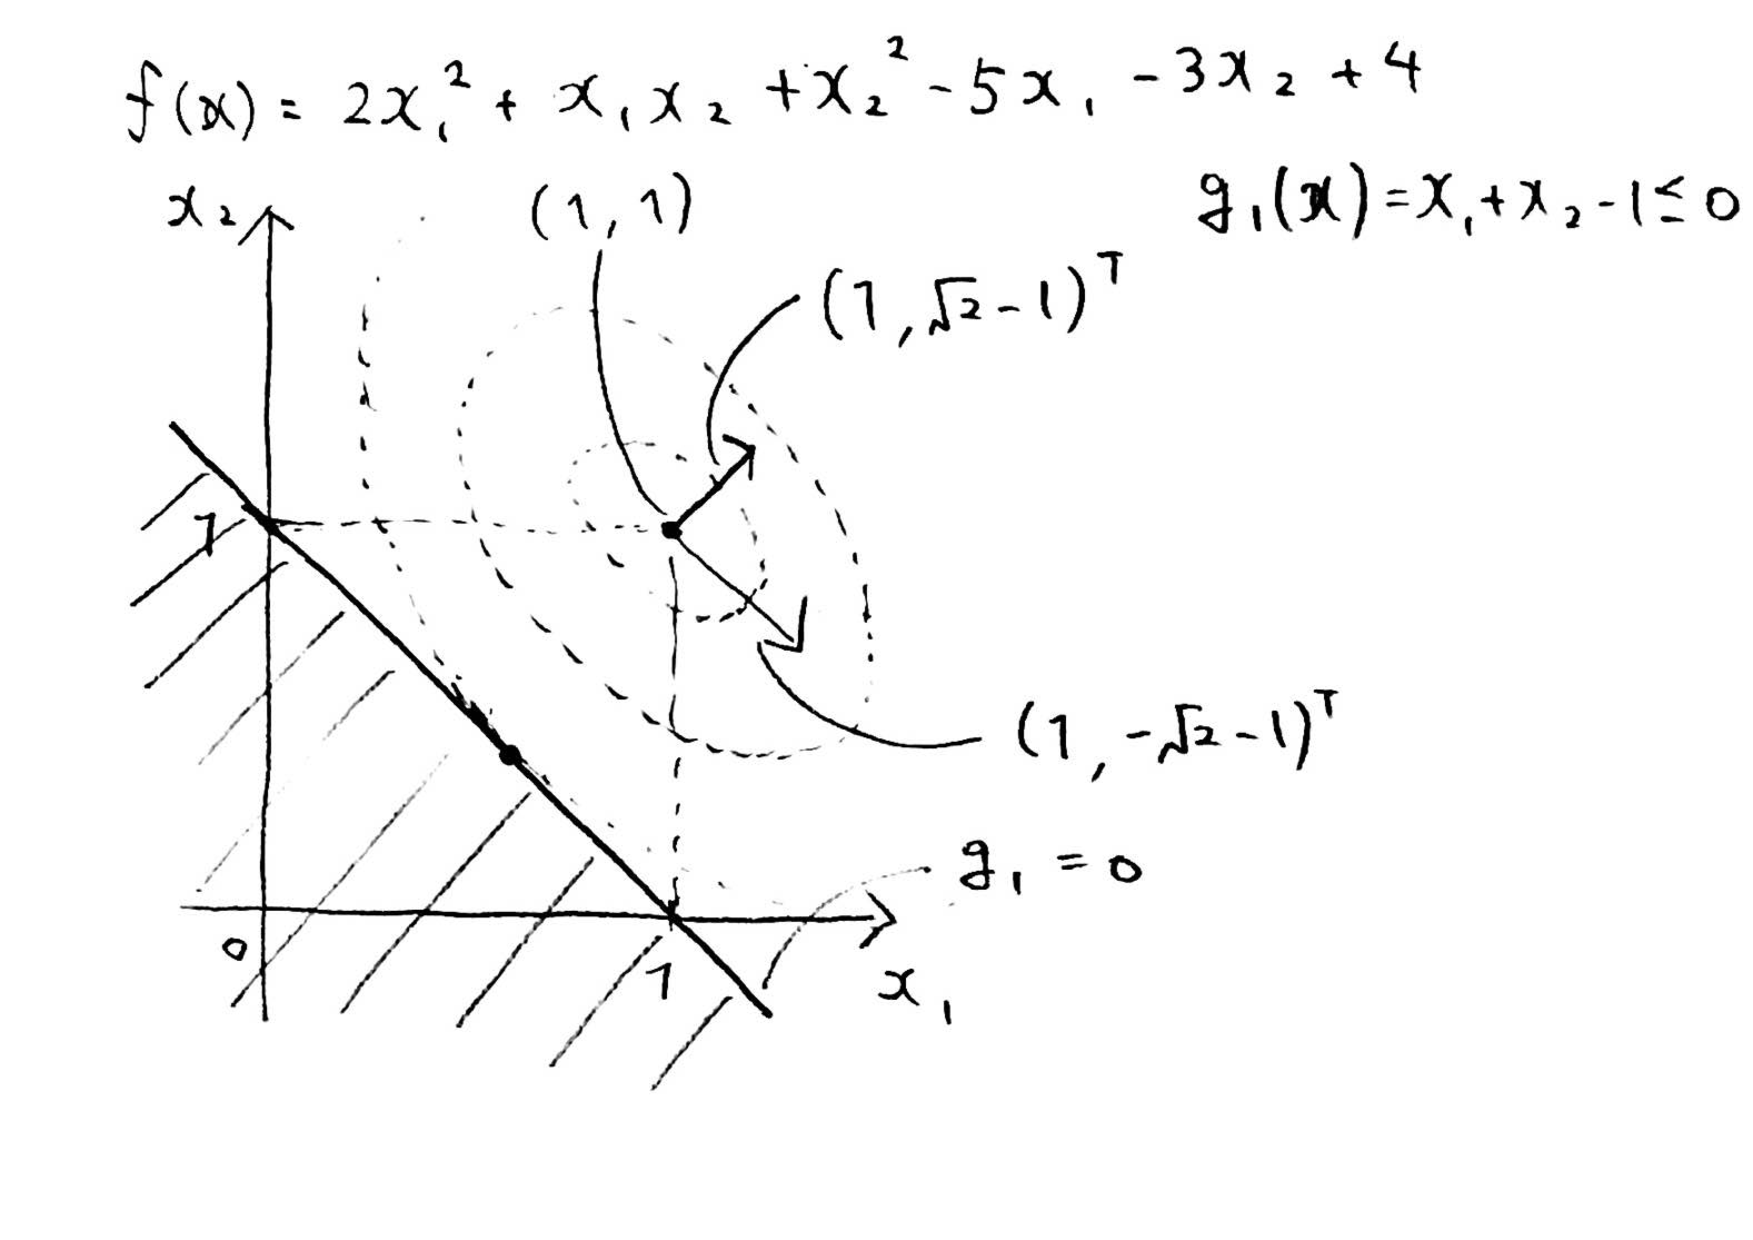
\includegraphics[clip, width=7cm]{../figure/KKT_3.pdf}
  \caption{実行可能領域と$f$の等高線}
  \label{fig:feasible_ex}
\end{figure}

$g_1(\bm{x})$は有効制約であると考えられる.よって,KKT条件は
\begin{align}
  &\left(
  \begin{array}{c}
    4x_1 + x_2 - 5 \\
    x_1 + 2x_2 - 3
  \end{array}
  \right) + u\left(
  \begin{array}{c}
    1 \\
    1
  \end{array}
  \right) = \left(
  \begin{array}{c}
    0 \\
    0
  \end{array}
  \right) \nonumber \\
  &x_1 + x_2 - 1 = 0 \nonumber
\end{align}
より,
\begin{equation}
  (\bar{x}_1, \bar{x}_2, u) = \left(\frac{3}{4}, \frac{1}{4}, \frac{7}{4} \right) \nonumber
\end{equation}
を得る.容易にわかるようにこれは最適解であり,最適値は
\begin{equation}
  f^{*} = \frac{7}{8} \nonumber
\end{equation}
である.

次に,この問題の双対問題を考える.Lagrange関数は,
\begin{equation}
  L(\bm{x}, u) = 2x_1^2 + x_1x_2 + x_2^2 + (u - 5)x_1 + (u - 3)x_2 + 4 - u \nonumber
\end{equation}
である.$u$を固定して$q(u)$を求めるため,停留点条件
\begin{equation}
  \nabla_{\bm{x}} L(\bm{x}, u) = \left(
  \begin{array}{c}
    4x_1 + x_2 + u - 5 \\
    x_1 + 2x_2 + u - 3
  \end{array}
  \right) = \left(
  \begin{array}{c}
    0 \\
    0
  \end{array}
  \right) \nonumber
\end{equation}
を解くと,
\begin{equation}
  x_1 = 1 - \frac{3}{7} u, \; x_2 = 1 - \frac{1}{7} u \nonumber
\end{equation}
を得る.この結果を$L(\bm{x}, u)$に代入して整理すると,
\begin{equation}
  q(u) = -\frac{2}{7} u^2 + u = - \frac{2}{7}\left(u - \frac{7}{4}\right)^2 + \frac{7}{8} \nonumber
\end{equation}
となる.したがって,双対問題は
\begin{align}
  \mathrm{maximize} \; \; &-\frac{2}{7} u^2 + u \nonumber\\
  \mathrm{subject \; to} \; \; &u \in \mathbb{R}_{+} \nonumber
\end{align}
と書ける.この問題の最適解は$u = 7/4$であり,最適値は
\begin{equation}
  q^{*} = \frac{7}{8} \nonumber
\end{equation}
である.以上をまとめ,$f^{*} = q^{*}$の成立が判明した.\qed

\paragraph{鞍点と最適性}
Lagrange関数$L(\bm{x}, \bm{u})$に対し,次の条件を満たす$\bm{x}^{*} \in X, \, \bm{u}^{*} \in \mathbb{R}_{+}^{m}$が存在するならば,$(\bm{x}^{*}, \bm{u}^{*})$を$L$の鞍点(saddle point)という.
\begin{equation}\label{eq:saddle}
  L(\bm{x}, \bm{u}^{*}) \geq L(\bm{x}^{*}, \bm{u}^{*}) \geq L(\bm{x}^{*}, \bm{u}), \; \forall \bm{x} \in X, \, \forall \bm{u} \in \mathbb{R}_{+}^{m}
\end{equation}

\begin{coro}
  主問題(\ref{eq:opt_nonl_f_true})と双対問題(\ref{eq:lag_dual})に対し,以下の条件はそれぞれ$\bm{x}^{*} \in X$が主問題の,$\bm{u}^{*}$が双対問題の最適解であるための十分条件である.
  \begin{enumerate}
    \item $\bm{x}^{*}$は主問題の実行可能解,$\bm{u}^{*}$は双対問題の実行可能解であり,さらに$f(\bm{x}^{*}) = q(\bm{u}^{*})$を満たす.
    \item $(\bm{x}^{*}, \bm{u}^{*})$はLagrange関数$L(\bm{x}, \bm{u})$の鞍点である.
  \end{enumerate}
\end{coro}

\paragraph{等式制約がある場合の双対問題}

\begin{align}\label{eq:opt_nonl_eq_dual}
  \mathrm{minimize} \; \; &f(\bm{x}) \nonumber\\
  \mathrm{subject \; to} \; \; &g_i(\bm{x}) \leq 0, \; i = 1, 2, \ldots, l \nonumber \\
  &g_i(\bm{x}) = 0, \; i = l+1, \ldots, m \\
  &\bm{x} \in X \nonumber
\end{align}

等式条件は,
\begin{equation}
  g_i(\bm{x}) \leq 0, \; -g_i(\bm{x}) \leq 0, \; i = l + 1, \ldots, m \nonumber
\end{equation}
と不等式の対で表し,対応するラグランジュ乗数をそれぞれ$u_i^{+}, \, u_i^{-}$と記すと,Lこの問題のLagrange関数は
\begin{equation}\label{eq:lag_eq}
  L(\bm{x}, \bm{u}) = f(\bm{x}) + \sum_{i = 1}^l u_i g_i(\bm{x}) + \sum_{i = l + 1}^{m}(u_i^{+} - u_i^{-})g_i(x)
\end{equation}
である.ただし,
$u_i \geq 0, i = 1, 2, \ldots, l, \; u_i^{+}, u_i^{-} \geq 0, i = l + 1, \ldots, m$
であるが,
\begin{equation}
  u_i = u_i^{+} - u_i^{-}, \; i = l + 1, \ldots, m
\end{equation}
とおくと,$u_i$は正負どちらの値もとることができて符号制約はなくなる.この$u_i$を用いると,LLこの問題のLagrange関数は
\begin{equation}
  L(\bm{x}, \bm{u}) = f(\bm{x}) + \sum_{i = 1}^m u_i g_i(\bm{x}) \nonumber
\end{equation}
ただし,
\begin{align}\label{eq:lag_u}
  &u_i \geq 0, \; i = 1, 2, \ldots, l \nonumber \\
  &u_i \, : \, 符号制限なし, \; i = l + 1, \ldots, m
\end{align}
となる.つまり,等式条件に対するラグランジュ乗数の符号制限がなくなる点だけが異なる.

この$L(\bm{x}, \bm{u})$から双対問題に至るまでは,不等式制約のみの議論をほぼそのまま適用することができる.得られる双対問題は,
\begin{align}\label{eq:dual_eq}
  \mathrm{maximize} \; \; &q(\bm{u}) \nonumber \\
  \mathrm{subject \; to} \; \; &\bm{u} \in \mathbb{R}^m \\
  &u_i \geq 0, \; i = 1, 2, \ldots, l \nonumber
\end{align}
である.弱双対定理\ref{theo:weak_dual}もそのまま成立する.

\section{凸計画問題の双対定理}
主問題として
\begin{align}\label{eq:opt_nonl_f_convex}
  \mathrm{minimize} \; \; &f(\bm{x}) \nonumber\\
  \mathrm{subject \; to} \; \; &g_i(\bm{x}) \leq 0, \; i = 1, 2, \ldots, m  \\
  &\bm{x} \in \mathbb{R}^n \nonumber
\end{align}
を考える.ただし,$f(\bm{x})$および$g_i(\bm{x}), \, i = 1, 2, \ldots, m$はすべて凸関数である.さらに,実行可能領域は内点$\bm{x}^{\prime} \in \mathbb{R}^n$を持つ(Slaterの制約想定).
\begin{equation}\label{eq:slater}
  g_i(\bm{x}^{\prime}) < 0, \; i = 1, 2, \ldots, m
\end{equation}
このとき,次の定理が成立する.
\begin{theo}[凸計画問題の双対定理]\label{theo:dual_convex}
  凸計画問題(\ref{eq:opt_nonl_f_convex})がSlaterの制約想定(\ref{eq:slater})を満たすと仮定し,最適値を$f^{*}$,その双対問題(\ref{eq:lag_dual})の最適値を$q^{*}$と記す.このとき,$f^{*} = q^{*}$が成立する.
\end{theo}



\end{document}


%%%%%%%%%%%% 証明 %%%%%%%%%%%%%%%%%%%%%%%%%%%%%%%%%%%%%%%%%%%%%%%%%%%
\documentclass[dvipdfmx]{jsreport}
\usepackage{graphicx, url, algorithm, algorithmic, float, booktabs, listings, color, pdfpages, amsmath, amssymb, latexsym, mathtools, ascmac, amsfonts, amsthm}
\lstset{
  basicstyle={\ttfamily},
  identifierstyle={\small},
  commentstyle={\smallitshape},
  keywordstyle={\small\bfseries},
  ndkeywordstyle={\small},
  stringstyle={\small\ttfamily},
  frame={tb},
  breaklines=true,
  columns=[l]{fullflexible},
  numbers=left,
  xrightmargin=0zw,
  xleftmargin=3zw,
  numberstyle={\scriptsize},
  stepnumber=1,
  numbersep=1zw,
  lineskip=-0.5ex
}
\usepackage[table,xcdraw]{xcolor}
\newtheorem{theo}{定理}[chapter]
\newtheorem{defi}{定義}[chapter]
\newtheorem{lemm}{補題}[chapter]
\newtheorem{prop}{命題}[chapter]
\newtheorem{coro}{系}[chapter]
\newcommand{\red}[1]{\textcolor{red}{#1}}
\newcommand{\blue}[1]{\textcolor{blue}{#1}}
\newcommand{\green}[1]{\textcolor{green}{#1}}
\renewcommand{\baselinestretch}{1.1}
\usepackage{mathrsfs}
\usepackage{bm}
\def\qed{\hfill $\Box$}
\usepackage{tikz}
\usetikzlibrary{intersections, calc, arrows}
\renewcommand\proofname{\bf 証明}

\begin{document}
\chapter{証明}
この付録には,補題や定理の証明を記載する.

\begin{proof}[補題\ref{lemm:convex}の証明]
  項が2つのとき,つまり,$X_1, X_2 \subseteq \mathbb{R}^n$が凸集合ならば,$X_1 \cap X_2$も凸集合である(*)
  を証明する.$\forall \bm{x}^1, \bm{x}^2 \in X_1 \cap X_2$に対し,$\bm{x}^1$と$\bm{x}^2$を結ぶ線分は,$\bm{x}^1 \in X_1, \bm{x}^2 \in X_1$より$X_1$に含まれる($\because$ $X_1$は凸集合).同様に$X_2$にも含まれる.
  よって,$\bm{x}^1$と$\bm{x}^2$を結ぶ線分は,$X_1 \cap X_2$に含まれる.つまり,$X_1 \cap X_2$は凸集合である.補題\ref{lemm:convex}は,(*)を繰り返し用いることで示される.\qed
\end{proof}

補題\ref{lemm:hyperplane1}の証明には,定理\ref{theo:projection},補題\ref{lemm:proj}を用いる.

\begin{theo}[射影定理]\label{theo:projection}
  $X$をHilbert空間\footnote{距離(ノルム)を持つ集合をノルム空間という.内積を持つ線形空間を内積空間という.ノルム空間$X$内の任意のコーシー列が収束するとき,$X$は完備であるといい,完備性を持つノルム空間$X$をBanach空間という.また,内積空間$X$上の点$\bm{u} \in X$に対し,$\|\bm{u}\| = \sqrt{(\bm{u}, \bm{u})}$を内積から誘導されるノルムと呼ぶ.内積から誘導されるノルム空間$X$がBanach空間であるとき,$X$をHilbert空間という.実数空間$\mathbb{R}^n$は完備性を持つ.}とし,$L \subset X$を閉部分空間とする.このとき,
  \begin{equation}
    \bm{u} \in X \, (\mathrm{given}) \Rightarrow \exists! \bm{v} \in L \; s.t. \; (\bm{u} - \bm{v}, \bm{w}) = 0, \, \forall \bm{w} \in L \nonumber
  \end{equation}
  が成立する(射影が一意に存在する).
\end{theo}

\begin{lemm}\label{lemm:proj}
    定理\ref{theo:projection}の$X$が$X = \mathbb{R}^n$であり,$L \subseteq \mathbb{R}^n$が空でない閉凸集合とする.$\bm{u} \in \mathbb{R}^n$の$L$への射影を$\bm{v}$とする.このとき,$\forall \bm{w} \in L$に対して,
  \begin{equation}\label{eq:proj}
    (\bm{u} - \bm{v})^{\mathrm{T}} (\bm{w} - \bm{v}) \leq 0
  \end{equation}
  が成立する.
\end{lemm}

\begin{proof}[定理\ref{theo:projection}の証明]

\end{proof}

\begin{proof}[補題\ref{lemm:proj}の証明]
  $\bm{u}$の$L$への射影$\bm{v}$と任意の点$\bm{w} \in L$を結ぶ線分上の点
  $\bm{x}_{\lambda} = (1 - \lambda)\bm{v} + \lambda \bm{w}, \, 0 < \lambda < 1$
  を考える.$L$は凸より,$\bm{x}_{\lambda}$も$L$に含まれる.
  $\bm{v}$の定義より,
  \begin{equation}\label{eq:prj_min}
    \|\bm{v} - \bm{u}\|^2 \leq \|((1 - \lambda)\bm{v} + \lambda \bm{w}) - \bm{u} \|^2
  \end{equation}
  (\ref{eq:prj_min})式を整理すると,
  \begin{align}
    (\bm{v}- \bm{u}, \bm{v}- \bm{u}) &\leq \|(\bm{v} - \bm{u}) + \lambda(\bm{w} - \bm{v}) \|^2 \nonumber \\
    &\leq (\bm{v}- \bm{u}, \bm{v}- \bm{u}) + 2\lambda(\bm{v} - \bm{u})(\bm{w} - \bm{v}) + \lambda^2(\bm{w} - \bm{v}, \bm{w} - \bm{v}) \nonumber
  \end{align}
  いま,$\lambda \neq 0, \lambda > 0$であり,$L \subseteq \mathbb{R}^n$であるから,
  \begin{equation}
    2(\bm{u} - \bm{v})(\bm{w} - \bm{v}) \leq \lambda \|\bm{w} - \bm{v}\|^2 \nonumber
  \end{equation}
  よって,$\lambda \rightarrow 0$とすると,(\ref{eq:proj})式を得る.\qed
\end{proof}

\begin{proof}[補題\ref{lemm:hyperplane1}の証明]
  $\bm{y}$の$X$への射影を$\bar{\bm{y}}$とする.$\bm{y} \notin X$より,$\bm{y} \neq \bar{\bm{y}}$である.
  よって,
  \begin{equation}\label{eq:norm}
    \|\bar{\bm{y}} - \bm{y}\|^2 = (\bar{\bm{y}} - \bm{y})^{\mathrm{T}}(\bar{\bm{y}} - \bm{y}) > 0
  \end{equation}
  である.また,補題\ref{lemm:proj}より,
  \begin{equation}\label{eq:prj}
    (\bm{y} - \bar{\bm{y}})^{\mathrm{T}}(\bm{x} - \bar{\bm{y}}) \leq 0, \; x \in X
  \end{equation}
  が成立する.(\ref{eq:norm})式,(\ref{eq:prj})式より,
  \begin{equation}
    (\bar{\bm{y}} - \bm{y})^{\mathrm{T}} \bm{x} \geq (\bar{\bm{y}} - \bm{y})^{\mathrm{T}} \bar{\bm{y}} > (\bar{\bm{y}} - \bm{y})^{\mathrm{T}} \bm{y}, \; x \in X \nonumber
  \end{equation}
  を得る.ここで,$\bm{a} = \bar{\bm{y}} - \bm{y}, \, b = (\bar{\bm{y}} - \bm{y})^{\mathrm{T}} \bar{\bm{y}}$と置くと補題\ref{lemm:hyperplane1}が示される.\qed
\end{proof}

\begin{proof}[補題\ref{lemm:hyperplane2}の証明]

\end{proof}

\begin{proof}[補題\ref{lemm:hyperplane3}の証明]

\end{proof}

\end{document}



\begin{thebibliography}{99}
\bibitem{or} オペレーションズ・リサーチとは. 公益社団法人日本オペレーションズ・リサーチ学会. https://www.orsj.or.jp/whatisor/whatisor.html. (参照 2020/3/23)
\bibitem{opt} 茨木俊秀. (2011). 最適化の数学. 共立出版株式会社.
\end{thebibliography}


\end{document}
